\chapter{Stable Neo-Hookean Flesh Simulation} \label{c:Paper}
In this chapter, I will examine further the topic of the paper \textit{\acrshort{snh}}. In the interest of understanding the thought process of the authors, I will include some of their calculations more detailed. In addition, examples and visualisations are presented for a better understanding. 

\section{Deformation Gradient}
In the following calculations the properties of the deformation gradient $\mathbf{F}$ covered in chapter 2 will be used. These properties are summarized in table \ref{table:gradient_quantities} for a better overview.

\begin{table}[!htbp]
\centering
    \begin{tabular}{ | l | l |}
    \hline
    \textbf{Symbol} & \textbf{Definition} \\ \hline
    $\mathbf{F} = \mathbf{RS}$ & Polar decomposition \\ \hline
    $J=\operatorname{det}(\mathbf{F})$ & Relative volume change \\ \hline
    $\mathbf{C}=\mathbf{F}^\intercal \mathbf{F}$ & Right Cauchy-Green  \\ \hline	
    $I_{C}=\operatorname{tr}(\mathbf{C})$ & First right Cauchy-Green invariant \\ \hline
    \end{tabular}
    \caption[Quantities derived from the Deformation Gradient]{Quantities derived from the Deformation Gradient}
\label{table:gradient_quantities}
\end{table}


\section{Energy Formulation}
\subsection{Stability}
The core goal of the paper was to model deformations for virtual characters that have human-like features. In order to achieve better results than what has been done in current research, they formulated a new deformation energy. In chapter 2, I concluded that the appropriate energy for animating soft tissues such as flesh has to be hyperelastic. An important property is the stability of the energy. We need an energy that is stable in the following four ways:

\textbf{1. Inversion Stability:} Given some arbitrary object, it is possible that while deforming the object we can arrive at a zero volume state or even an entire inversion. Take for example the tetrahedron shown in Fig. \ref{fig:inversion_1}. In Fig. \ref{fig:inversion_2} we see a deformed state of this tetrahedron where the volume is scaled down to zero and we are left with a simple triangle. In Fig. \ref{fig:inversion_3} the tetrahedron arrives at an inversed stated. The deformation energy has to be able to deal with both cases without creating severe artefacts. That means, that the energy has to be singularity-free, meaning that it is defined for every possible point. This should hold without needing any filters or threshold (\cite{Smith:2018:SNF:3191713.3180491}, 12:3).

\begin{figure}[!ht]
\centering
\begin{subfigure}{.3\textwidth}
  \centering
  % include first image
  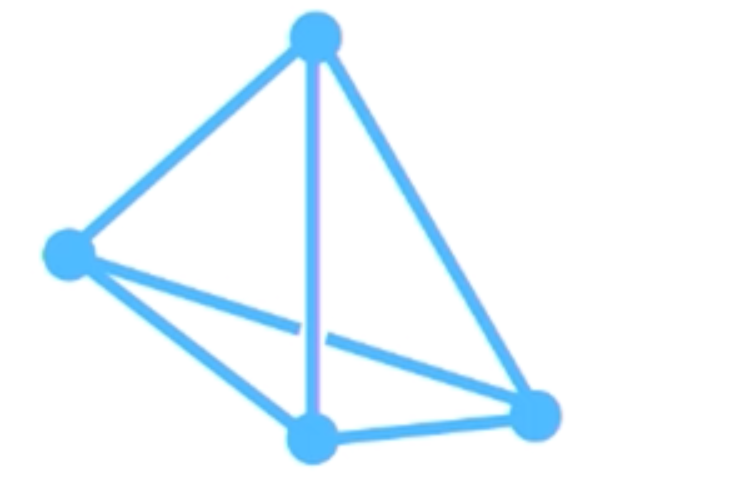
\includegraphics[width=.8\linewidth]{resources/inversion_1}  
  \caption{Rest state}
  \label{fig:inversion_1}
\end{subfigure}
\begin{subfigure}{.3\textwidth}
  \centering
  % include first image
  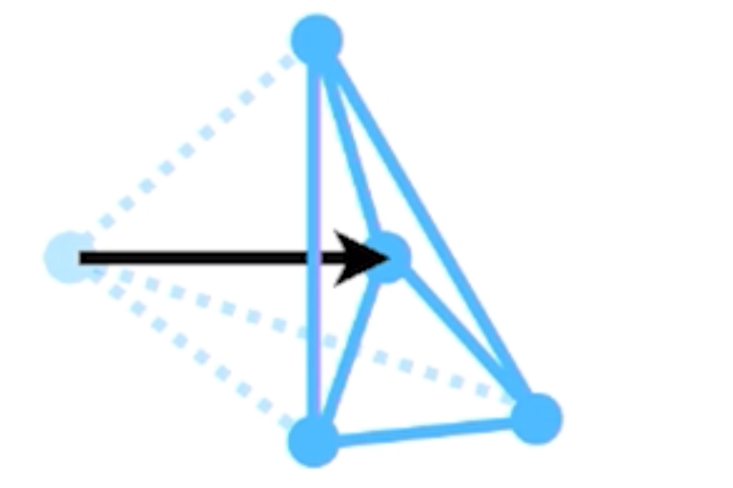
\includegraphics[width=.8\linewidth]{resources/inversion_2}  
  \caption{Zero-volume state}
  \label{fig:inversion_2}
\end{subfigure}
\begin{subfigure}{.3\textwidth}
  \centering
  % include second image
  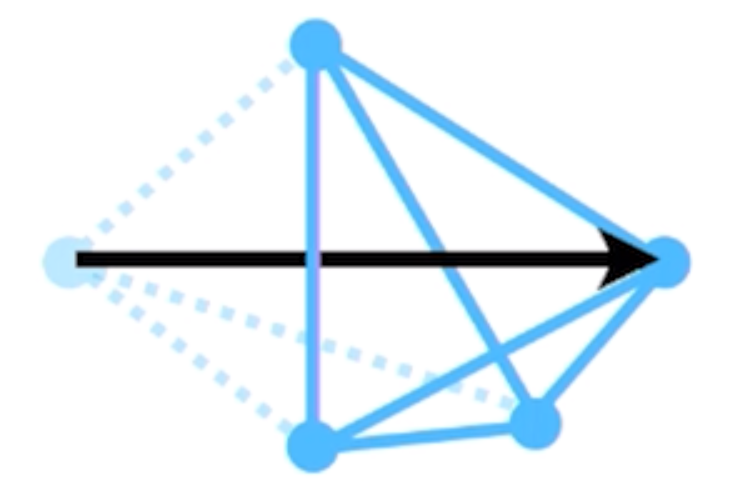
\includegraphics[width=.8\linewidth]{resources/inversion_3}  
  \caption{Inversed state}
  \label{fig:inversion_3}
\end{subfigure}
\caption[Inversion of a tetrahedron]{Inversion of a tetrahedron {\cite{STREAM2018}}}
\label{fig:inversion}
\end{figure}


\textbf{2. Reflection stability:} While deforming an object, it can occur that we are dealing with reflections. An example of a reflection in 2D is shown in Fig. \ref{fig:reflection}. Here the coloured triangle is reflected over the y-axis. A matrix that represents a reflection is orthogonal with determinant $-1$. The deformation energy needs to be well behaved under reflections. This has to hold, regardless of the reflection convention used in the \acrshort{svd} of \textbf{F}. The reflection convention is explained in chapter 2.3.2 in the subsection \textit{Singular Value Decomposition of \textbf{F}}.

\begin{figure}[!htbp]
	\centering
	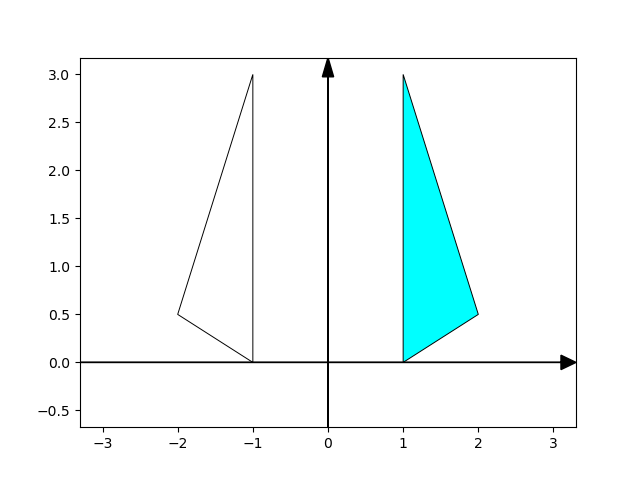
\includegraphics[width=0.5\textwidth]{resources/reflection_plot.png}
	\caption[Reflection of a triangle over the y-axis]{Reflection of a triangle over the y-axis}
	\label{fig:reflection}
\end{figure}

\textbf{3. Rest stability:} When deforming an object in a certain way, we apply one or multiple forces to that object, which influences the deformation. But when we remove all the forces, the object should be back in its rest state.

\textbf{4. Meta-stability under degeneracy:} This is a special case of rest stability. We can crush an object into an arbitrary shape like a plane, line or point. This process is illustrated for a cube in Fig. \ref{fig:meta_stability}. Afterwards, when the applied forces are removed, the cube should still be able to recover from this arbitrary shape to its actual shape.

\begin{figure}[!htbp]
	\centering
	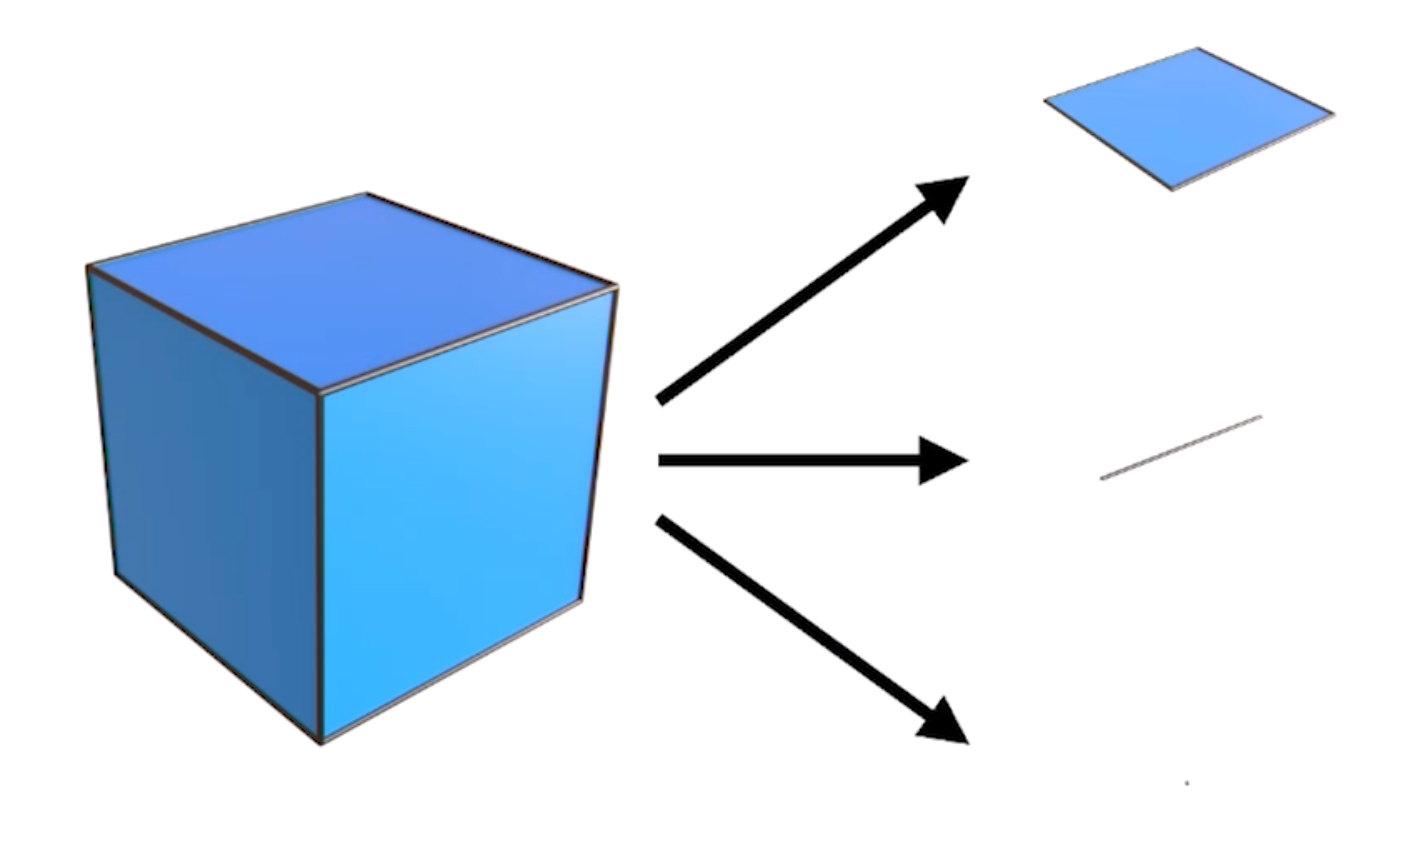
\includegraphics[width=0.5\textwidth]{resources/meta_stability}
	\caption[Illustration of meta stability]{Illustration of meta stability {\cite{STREAM2018}}}
	\label{fig:meta_stability}
\end{figure}

Based on these four requirements, we will determine if a deformation energy is suited for our needs.

\todoredefined[inline]{
TODO: Are images ok?
}


\subsection{Existing Neo-Hookean Energies}

In previous literature, a few energies were proposed that I will analyse in this section. They are listed in table \ref{table:energies}.

\begin{table}[!htbp]
\centering
    \begin{tabular}{ | l | l |}
    \hline
    \textbf{Energy} & \textbf{Author(s)} \\ \hline
    $\Psi_{Neo}=\frac{\mu}{2}\left(I_{C}-3\right)-\mu \log J+\frac{\lambda}{2}(\log J)^{2}$ & \begin{tabular}{@{}l@{}}e.g. Bonet and Wood 1997 \\ (\cite{bonet1997nonlinear})\end{tabular}  \\ \hline
    $\Psi_{\mathrm{A}}=\frac{\mu}{2}\left(I_{C}-3\right)-\mu \log J+\frac{\lambda}{2}(J-1)^{2}$ & Odgen 1997 (\cite{ogden1997non}) \\ \hline
    $\Psi_{\mathrm{B}}=\frac{\mu}{2}\left(J^{-2 / 3} I_{C}-3\right)+\frac{\lambda}{2}(J-1)^{2}$ & Bower 2009 (\cite{bower2009applied}) \\ \hline
    $\Psi_{\mathrm{C}}=\frac{\mu}{2}\left(J^{-2 / 3} I_{C}-3\right)+\frac{\lambda}{2}(J-1)^{2}$ & \begin{tabular}{@{}l@{}}Wang and Yang 2016 \\ (\cite{wang2016descent}) \end{tabular} \\ \hline
    \end{tabular}
    \caption[Summary of proposed energies]{Summary of proposed energies (\cite{Smith:2018:SNF:3191713.3180491}, 12:3)}
\label{table:energies}
\end{table}

Each energy formulation can be split up into a 1D length term and a 3D volume term. The 1D length term penalizes the length changes an object undergoes, whereas the 3D volume term is a volume-preserving penalty term.

\begin{table}[!htbp]
\centering
    \begin{tabular}{ | l | l | l |}
    \hline
    \textbf{Energy} & \textbf{1D length term} & \textbf{3D volume term} \\ \hline
    $\Psi_{Neo}$ & $\frac{\mu}{2}\left(I_{C}-3\right)$ & $-\mu \log J+\frac{\lambda}{2}(\log J)^{2}$ \\ \hline
    $\Psi_{\mathrm{A}}$ & $\frac{\mu}{2}\left(I_{C}-3\right)$ & $-\mu \log J+\frac{\lambda}{2}(J-1)^{2}$ \\ \hline
    $\Psi_{\mathrm{B}}$ & $\frac{\mu}{2}\left(J^{-2 / 3} I_{C}-3\right)$ & $\frac{\lambda}{2}(J-1)^{2}$ \\ \hline
    $\Psi_{\mathrm{C}}$ & $\frac{\mu}{2}\left(J^{-2 / 3} I_{C}-3\right)$ & $\frac{\lambda}{2}(J-1)^{2}$ \\ \hline
    \end{tabular}
    \caption{Energies split up into their 1D length and 3D volume term}
\label{table:energies_split}
\end{table}

\subsubsection{1D Length Term}
Mooney (\cite{mooney1940theory}) originally proposed the 1D length term 
\[
\Psi_{M}=\frac{\mu}{2}\left(I_{C}-3\right),
\]
which is used in $\Psi_{Neo}$ and $\Psi_{A}$. If we expand the energy with the singular values of the deformation gradient \textbf{F}, we get the following term:
\[
\Psi_{M}=\frac{\mu}{2}\left(\sigma_{0}^2 + \sigma_{1}^2 + \sigma_{2}^2 - 3\right)
\]
This energy reaches its minimum at a zero volume state, meaning $I_{C}=0$. Mooney added the hard constraint that $J$ should be equal to $1$, so that the energy is minimized at the volume preserving configuration that is closest to the stretch space origin. Note that the energy is singularity free and well defined under inversion.

The second term is
\[
\Psi_{R} = \frac{\mu}{2}\left(J^{-2 / 3} I_{C}-3\right)
\]
and used in $\Psi_{B}$ and $\Psi_{C}$ and was introduced by Rivlin (\cite{rivlin1948large}). Using the singular values of \textbf{F}, we get the following term:
\[
\Psi_{R} = \frac{\mu}{2}\left(\frac{\sigma_{0}^2 + \sigma_{1}^2 + \sigma_{2}^2}{(\sigma_{0}  \sigma_{1}  \sigma_{2})^\frac{2}{3}}
 - 3\right)
\]
Unfortunately, this term is not singularity free. If either $\sigma_{0}$, $\sigma_{1}$ or $\sigma_{2}$ is equal to zero the result is not defined anymore.

\subsubsection{3D Volume Term}
The volume term of $\Psi_{Neo}$, meaning
\[
\Psi_{Neo, volume} = -\mu \log J+\frac{\lambda}{2}(\log J)^{2},
\]
results in numerical problems, since the logarithmic function is not defined for $J<0$ and grows unbounded for $J \rightarrow 0$. In conclusion, $\Psi_{Neo, volume}$ is not singularity free. 
The same applies for the 3D volume term of $\Psi_{A}$, namely
\[
\Psi_{A, volume} = -\mu \log J+\frac{\lambda}{2}(J-1)^{2}.
\]
The term of $\Psi_{A}$ and $\Psi_{B}$, which is of the form
\[
\Psi_{M} = \frac{\lambda}{2}(J-1)^{2},
\]
does not have these problems. It is bounded, well defined and invertible. After these observations we combine the robust length with the robust volume term and receive $\Psi_D$, which is defined as
\[
\Psi_{D} = \frac{\mu}{2}\left(I_{C}-3\right) +\frac{\lambda}{2}(J-1)^{2}.
\]
$\Psi_{D}$ is singularity free and well defined under inversion. Unfortunately, it does not satisfy the requirement of being rest stable, which will be discussed in the next section.

\todoredefined[inline]{
TODO: explain how to get to equation with singular values?
}

\subsection{Rest Stabilization}
Although $\Psi_{D}$ meets almost all stated requirements, it is not rest stable. This can be shown with the first Piola-Kirchhoff (PK1) stress tensor, defined as $\Psi_D$ derived by the deformation gradient \textbf{F}:
\begin{align*}
P_{D}(\mathbf{I}) &= \frac{\partial \Psi_{D}}{\partial \mathbf{F}} (\mathbf{I}) = \frac{\partial \Psi_{D}}{\partial \mathbf{F}} \left[ \frac{\mu}{2}\left(I_{C}-3\right) +\frac{\lambda}{2}(J-1)^{2} \right] \\
&= \frac{\partial \Psi_{D}}{\partial \mathbf{F}}  \frac{\mu}{2}\left(\operatorname{tr}(\mathbf{I}^\intercal \mathbf{I})-3\right) +\frac{\partial \Psi_{D}}{\partial \mathbf{F}} \frac{\lambda}{2}(\operatorname{tr}(\mathbf{I})-1)^{2} \\
&= \mu \mathbf{I} + \lambda (\operatorname{det}(\mathbf{I})-1)  \frac{\partial}{\partial \mathbf{F}} \operatorname{det}(\mathbf{I}) = \mu \mathbf{I} \neq 0
\end{align*}

If the energy had rest stability, $P_{D}(\mathbf{I})$ would resolve to zero. Unfortunately, this is not the case here. In order to solve this problem, the authors modified $(J-1)^{2}$ to $(J-\alpha)^{2}$. Using this modification, the energy can be written as
\[
\Psi_{E} = \frac{\mu}{2}\left(I_{C}-3\right) +\frac{\lambda}{2}(J-\alpha)^{2}.
\]

Inserting $\Psi_E$ into the PK1 equation from before, we get
\begin{align*}
P_{E}(\mathbf{F}) &= \frac{\partial \Psi_{E}}{\partial \mathbf{F}} \left[ \frac{\mu}{2}\left(I_{C}-3\right) +\frac{\lambda}{2}(J-\alpha)^{2} \right] \\
&= \mu \mathbf{F} + \lambda (\operatorname{det}(\mathbf{F})-\alpha)  \frac{\partial}{\partial \mathbf{F}} \operatorname{det}(\mathbf{F}).
\end{align*}
Solving for an alpha that satisfies $P_{E}(\mathbf{I})=0$ gives us $\alpha=1+\frac{\mu}{\lambda}$. Now $\Psi_{E}$ has to be changed accordingly:
\begin{align*}
\Psi_{E} &= \frac{\mu}{2}\left(I_{C}-3\right) +\frac{\lambda}{2}(J-1-\frac{\mu}{\lambda})^{2} \\
&= \frac{\mu}{2}\left(I_{C}-3\right) - \mu\left(J-1\right) + \frac{\lambda}{2}(J-1)^{2} + \left(\frac{\mu}{\lambda}\right)^{2}.
\end{align*}
Since constants disappear under differentiation, this expression is functionally equivalent to 
\[
\Psi_{E} = \frac{\mu}{2}\left(I_{C}-3\right) - \mu\left(J-1\right) + \frac{\lambda}{2}(J-1)^{2}.
\]
Note that $\Psi_{E}$ looks very similar to $\Psi_{Neo}$. The difference is that $log(J)$ is replaced with $(J-1)$ in $\Psi_{E}$. Keep in mind that $(J-1)$ is the first term in the taylor approximation of $\operatorname{log}(J)$ at $J=1$:
\begin{align*}
\sum_{n=0}^{\infty} &= \frac{f^{(n)}(1)}{n!} (J-1)^{n} \\
&= \boldsymbol{(J-1)} - \frac{1}{2} (J-1)^{2} + \frac{1}{3} (J-1)^{3} -\frac{1}{4} (J-1)^{4} + \text{...}
\end{align*}
Thus $\Psi_{E}$ is an approximation of $\Psi_{Neo}$.

\todoredefined[inline]{
TODO: Include all calculations? Check consistency of calculations (when trace when $I_C$ etc.).
}

\subsection{Meta-Stability under Degeneracy}
We have seen that he energy $\Psi_{E}$ has inversion, reflection and rest stability. Now we are interested in how it behaves under degeneracy. The authors of the paper \textit{\acrshort{snh}} viewed this as a Drucker stability analysis (see \cite{bower2009applied}). By Drucker stability, we mean a set of criteria that a material can satisfy or not. This is a measurement of the stability of the material. The calculations can be found in the supplemental material of \textit{\acrshort{snh}}, I will only present the results here. 

The energy remains stable when crushing the object into a \textit{plane}. The object is able to return to its rest state. Thus, no further adjustments need to be done. When crushing the object into a \textit{line}, the energy is meta-stable. A meta-stable state is a weaker state of stability that is resistant to small changes but not to large ones. The alternative would be a state that yields singularities, which worsens the situation. Hence, we can leave the energy as it is. After crushing the object to a \textit{point}, the material cannot recover into its rest state. This effect is small for a higher poisson's ratio. For completeness the authors nevertheless added a regularized origin barrier:
\[
	\Psi_{origin} = \operatorname{log}(I_C +\delta)
\]
This term eliminates the point meta-stability for a positive poisson's ratio, without interfering with the other requirements for the energy. It can be shown that the value $\delta$ should be set to $1$. This is also included in the supplemental material of the paper (\cite{Smith:2018:SNF:3191713.3180491}, 12:4).

The final energy is then
\begin{equation}\label{eq:stable_energy}
\Psi_{new} = \frac{\mu}{2}\left(I_{C}-3\right) + \frac{\lambda}{2}(J-\alpha)^{2} - \frac{\mu}{2} \operatorname{log}\left(I_{C}+1\right).
\end{equation}
With that adjustment the rest stability term can be written as $\alpha=1+\frac{\mu}{\lambda}-\left(\frac{\mu}{4}\right)\lambda$.

\subsection{Lamé Reparametrization}
In order to stay consistent with Hooke's law, we need to do a reparametrization of $\mu$ and $\lambda$. For achieving this, we set
\begin{equation}
	\mathbf{P}(\mathbf{F}) = 2 \mu_{Lamé} \epsilon + \lambda_{Lamé} \operatorname{tr}(\epsilon) \mathbf{I},
\end{equation}
where $\epsilon = \frac{1}{2} (\mathbf{F} + \mathbf{F}^\intercal) - \mathbf{I}$ is the linearized strain tensor. We then set $\mu = \frac{4}{3} \mu_{Lamé}$ and $\lambda = \lambda_{Lamé} + \frac{5}{6} \mu_{Lamé}$. The equation for the poisson's ratio then shifts to 
\[
	v= \frac{\lambda - \left( \frac{5}{8} \right) \mu}{2 \left(\lambda + \left( \frac{1}{8} \mu \right) \right)}.
\]

\todoredefined[inline]{
TODO: Do a better job here.
}


\section{Energy Analysis}
The goal of this chapter is to show that a complete eigenanalysis can be performed on Eq. \ref{eq:stable_energy}. This helps us understand the properties and limitations of the new energy.


\subsection{First Piola-Kirchhoff Stress (PK1)}
In order to analyse the energy, PK1 can be used for Eq. \ref{eq:stable_energy} with $\alpha=1+\frac{\mu}{\lambda}-\left(\frac{\mu}{4}\right)\lambda$:
\begin{align*}
P(\mathbf{F}) &= \frac{\partial \Psi_{D}}{\partial \mathbf{F}} \left[ \frac{\mu}{2}\left(I_{C}-3\right) + \frac{\lambda}{2}(J-\alpha)^{2} - \frac{\mu}{2}\left(I_{C}+1\right) \right] \\
&= \mu \mathbf{F} + \lambda (\operatorname{det}(\mathbf{F})-\alpha)  \frac{\partial}{\partial \mathbf{F}} \operatorname{det}(\mathbf{F}) - \frac{\partial}{\partial \mathbf{F}} \left[\operatorname{log}\left(\operatorname{tr}(\mathbf{F}^\intercal \mathbf{F})+1\right)\right] \\
&= \mu \mathbf{F} + \lambda (\operatorname{det}(\mathbf{F})-\alpha)  \frac{\partial}{\partial \mathbf{F}} \operatorname{det}(\mathbf{F}) - \mu \mathbf{F} \frac{1}{\operatorname{tr}(\mathbf{F}^\intercal \mathbf{F}) + 1} \\
&= \mu \left( 1 - \frac{1}{\operatorname{tr}(\mathbf{F}^\intercal \mathbf{F}) + 1}\right) \mathbf{F} + \lambda(J-\alpha)\frac{\partial J}{\partial \mathbf{F}}
\end{align*}

For further use it can be more practical to write $\frac{\partial J}{\partial \mathbf{F}}$ as a result of cross products:
\begin{equation}\label{eq:cross_product}
\frac{\partial J}{\partial \mathbf{F}} = \left[ \,f_1 \times f_2\, \bigg| \,f_2 \times f_0\, \bigg| \,f_0 \times f_1\, \right].
\end{equation}

\todoredefined[inline]{
TODO: Is it easy to follow? Maybe add some explanations of some steps?
}

\subsection{The Energy Hessian Terms}
Using the scalar notation for $\mathbf{F}$, the Hessian of the energy can be written as a fourth-order matrix-of-matrices:
\[
\frac{\partial^2 \psi}{\partial \mathbf{F}^2} = \frac{\partial P(\mathbf{F})}{\partial \mathbf{F}} = 
\left[\begin{array}{ccc}{\left[\frac{\partial P(\mathbf{F})}{\partial f_0}\right]} & {\left[\frac{\partial P(\mathbf{F})}{\partial f_3}\right]} & {\left[\frac{\partial P(\mathbf{F})}{\partial f_6}\right]} \\ {\left[\frac{\partial P(\mathbf{F})}{\partial f_1}\right]} & {\left[\frac{\partial P(\mathbf{F})}{\partial f_4}\right]} & {\left[\frac{\partial P(\mathbf{F})}{\partial f_7}\right]} \\ {\left[\frac{\partial P(\mathbf{F})}{\partial f_2}\right]} & {\left[\frac{\partial P(\mathbf{F})}{\partial f_5}\right]} & {\left[\frac{\partial P(\mathbf{F})}{\partial f_8}\right]} \end{array}\right]
\]

Each entry of the Hessian is defined as
\[
\frac{\partial P(\mathbf{F})}{\partial f_i} = \frac{\partial}{\partial f_i} \left[ \mu \left( 1 - \frac{1}{\operatorname{tr}(\mathbf{F}^\intercal \mathbf{F}) + 1}\right) \mathbf{F} + \lambda(J-\alpha)\frac{\partial J}{\partial \mathbf{F}} \right]
\]
\[
\stackrel{\text{prod.rule}}{=} \underbrace{\frac{\partial \mathbf{F}}{\partial f_i} \mu \left( 1 - \frac{1}{\operatorname{tr}(\mathbf{F}^\intercal \mathbf{F}) + 1}\right)}_{\mathrm{T}_{i}}  + \underbrace{\mathbf{F} \mu \frac{2}{\left(\operatorname{tr}(\mathbf{F^\intercal}\mathbf{F}) + 1\right)^2} f_i}_{_{\mathrm{M}_{i}}}
\]
\[
r+ \underbrace{\lambda \frac{\partial J}{\partial f_i} \frac{\partial J}{\partial \mathbf{F}}}_{_{\mathrm{G}_{i}}}+ \underbrace{\lambda (J- \alpha) \frac{\partial^2 J}{\partial \mathbf{F}\partial f_i}}_{_{\mathrm{H}_{i}}} \in \mathbb{R}^{3}.
\]
We can split up this final equation into these four term: $\mathrm{T}_i$ (Tikohonov), $\mathrm{M}_i$ (Mu), $\mathrm{G}_i$ (Volume Gradient), $\mathrm{H}_i$ (Volume Hessian). I will examine them separately in the next section.

\subsection{The Tikhonov, Mu, and Gradient Terms}
\subsubsection{Tikhonov}
The Tikhonov term is a fourth-order matrix-of-matrices. It is calculated by $\frac{\partial \mathbf{F}}{\partial f_i}$ and takes on the form
\[
\mathbb{T} = \left[\begin{array}{ccc}{\begin{bmatrix} 1 & 0 & 0 \\ 0 & 0 & 0 \\ 0 & 0 & 0 \end{bmatrix}} & {\begin{bmatrix} 0 & 1 & 0 \\ 0 & 0 & 0 \\ 0 & 0 & 0 \end{bmatrix}} & {\begin{bmatrix} 0 & 0 & 1 \\ 0 & 0 & 0 \\ 0 & 0 & 0 \end{bmatrix}} \\ {\begin{bmatrix} 0 & 0 & 0 \\ 1 & 0 & 0 \\ 0 & 0 & 0 \end{bmatrix}} & {\begin{bmatrix} 0 & 0 & 0 \\ 0 & 1 & 0 \\ 0 & 0 & 0 \end{bmatrix}} & {\begin{bmatrix} 0 & 0 & 0 \\ 0 & 0 & 1 \\ 0 & 0 & 0 \end{bmatrix}} \\ {\begin{bmatrix} 0 & 0 & 0 \\ 0 & 0 & 0 \\ 1 & 0 & 0 \end{bmatrix}} & {\begin{bmatrix} 0 & 0 & 0 \\ 0 & 0 & 0 \\ 0 & 1 & 0 \end{bmatrix}} & {\begin{bmatrix} 0 & 0 & 0 \\ 0 & 0 & 0 \\ 0 & 0 & 1 \end{bmatrix}} \end{array}\right].
\]
If we vectorize $\mathbb{T}$, we get the identity matrix $\mathbf{I} \in \mathbb{R}^{9x9}$ which is of full rank, positive definite and independent of the values in \textbf{F}: 
\[
\operatorname{vec}(\mathbb{T}) =  \mathbf{\check{T}} = \mathbf{I} = \in \mathbb{R}^{9x9}
\]
The Tikhonov term serves as a regularizer for the rest of the energy.

\subsubsection{Mu}
The Mu term has the same structure with different entries. It can be obtained by $\mathbf{F} f_i$ and has the form
\[
\mathbb{M} = \left[\begin{array}{ccc}{\begin{bmatrix} f_0^2 & f_0f_3 & f_0f_6 \\ f_0f_1 & f_0f_4 & f_0f_7 \\ f_0f_2 & f_0f_5 & f_0f_8 \end{bmatrix}} & {\begin{bmatrix} f_3f_0 & f_3^2 & f_3f_6 \\ f_3f_1 & f_3f_4 & f_3f_7 \\ f_3f_2 & f_3f_5 & f_3f_8 \end{bmatrix}} & {\begin{bmatrix} f_6f_0 & f_6f_3 & f_6f_6 \\ f_6f_1 & f_6f_4 & f_6f_7 \\ f_6f_2 & f_6f_5 & f_6f_8 \end{bmatrix}} \\ {\begin{bmatrix} f_1f_0 & f_1f_3 & f_1f_6 \\ f_1^2 & f_1f_4 & f_1f_7 \\ f_1f_2 & f_1f_5 & f_1f_8 \end{bmatrix}} & {\begin{bmatrix} f_4f_0 & f_4f_3 & f_4f_6 \\ f_4f_1 & f_4^2 & f_4f_7 \\ f_4f_2 & f_4f_5 & f_4f_8 \end{bmatrix}} & {\begin{bmatrix} f_7f_0 & f_7f_3 & f_7f_6 \\ f_7f_1 & f_7f_4 & f_7^2 \\ f_7f_2 & f_7f_5 & f_7f_8 \end{bmatrix}} \\ {\begin{bmatrix} f_2f_0 & f_2f_3 & f_2f_6 \\ f_2f_1 & f_2f_4 & f_2f_7 \\ f_2^2 & f_2f_5 & f_2f_8 \end{bmatrix}} & {\begin{bmatrix} f_5f_0 & f_5f_3 & f_5f_6 \\ f_5f_1 & f_5f_4 & f_5f_7 \\ f_5f_2 & f_5^2 & f_5f_8 \end{bmatrix}} & {\begin{bmatrix} f_8f_0 & f_8f_3 & f_8f_6 \\ f_8f_1 & f_8f_4 & f_8f_7 \\ f_8f_2 & f_8f_5 & f_8^2 \end{bmatrix}} \end{array}\right].
\]
When vectorizing $\mathbb{M}$, the resulting matrix $\mathbf{\check{M}}$ has the squared values of $f_i$ placed on the diagonal:
\[
\operatorname{vec}(\mathbb{M})= \mathbf{\check{M}} = \begin{bmatrix} f_0^2 & f_1f_0 & f_2f_0 & f_3f_0 & f_4f_0 & f_5f_0 & f_6f_0 & f_7f_0 & f_8f_0 \\ f_0f_1 & f_1^2 & f_2f_1 & f_3f_1 & f_4f_1 & f_5f_1 & f_6f_1 & f_7f_1 & f_8f_1 \\ f_0f_2 & f_1f_2 & f_2^2 & f_3f_2 & f_4f_2 & f_5f_2 & f_6f_2 & f_7f_2 & f_8f_2 \\ f_0f_3 & f_1f_3 & f_2f_3 & f_3^2 & f_4f_3 & f_5f_3 & f_6f_3 & f_7f_3 & f_8f_3 \\ f_0f_4 & f_1f_4 & f_2f_4 & f_3f_4 & f_4^2 & f_5f_4 & f_6f_4 & f_7f_4 & f_8f_4 \\ f_0f_5 & f_1f_5 & f_2f_5 & f_3f_5 & f_4f_5 & f_5^2 & f_6f_5 & f_7f_5 & f_8f_5 \\ f_0f_6 & f_1f_6 & f_2f_6 & f_3f_6 & f_4f_6 & f_5f_6 & f_6^2 & f_7f_6 & f_8f_6 \\ f_0f_7 & f_1f_7 & f_2f_7 & f_3f_7 & f_4f_7 & f_5f_7 & f_6f_7 & f_7^2 & f_8f_7 \\ f_0f_8 & f_1f_8 & f_2f_8 & f_3f_8 & f_4f_8 & f_5f_8 & f_6f_8 & f_7f_8 & f_8^2 \end{bmatrix}
\]
This structure makes it possible to write $\mathbf{\check{M}}$ as an outer product of $\operatorname{vec}(\mathbf{F})$:
\[
\mathbf{\check{M}}= \operatorname{vec}(\mathbf{F})\operatorname{vec}(\mathbf{F})^\intercal = \mathbf{\check{f}} \mathbf{\check{f}}^\intercal
\]
This matrix has rank one and has a single non-zero eigenvalue. In order to examine the eigenvalues, we can calculate
\[
\| \mathbf{\check{f}} \|^{2}_{2} = \sum_{n=0}^8 | f_n |^2 = \| \mathbf{F} \|^{2}_{F} = \sum_{n=0}^3 \sigma^2_i = \left( \sigma_0^2 + \sigma_1^2 + \sigma_2^2 \right),
\]
in which $\|\cdot\|_F$ stands for the Frobenius norm introduced in Def. \ref{FN} and $\sigma_i$ for the singular values from $\mathbf{\Sigma}$ in the \acrshort{svd} of $\mathbf{F}$ stated in Eq. \ref{eq:svd_simga}. The equation can be obtained by using Eq. \ref{eq:FN}, explained in chapter 2. The eigenvector is $\mathbf{\check{f}} / \| \mathbf{\check{f}} \|$. The eigenvalue is always non-negative and large if $\mathbf{F}$ contains a large strech.

\subsubsection{Gradient}
The gradient term also has the same structure as the two terms before with different entries defined by
\[
\mathbb{G}(\mathbf{F}) = \frac{\partial J}{\partial \mathbf{F}} \frac{\partial J}{\partial fi}.
\]
The vectorized matrix $\mathbf{\check{G}}$ can be written in a similar form as for the Mu term. With the help of the cross product of $\partial J / \partial \mathbf{F}$ stated in Eq. \ref{eq:cross_product}, $\mathbf{\check{G}}$ can be written as an outer product in the following way:
\[
\operatorname{vec}(\mathbb{G}(\mathbf{F})) = \mathbf{\check{G}} = \operatorname{vec}\left(\frac{\partial J}{\partial \mathbf{F}}\right) \operatorname{vec}\left(\frac{\partial J}{\partial \mathbf{F}}\right)^\intercal = \mathbf{\check{g}} \mathbf{\check{g}}^\intercal.
\]
As in the Mu term, we again have a single non-zero, non-negative eigenvalue calculated by
\[
\| \mathbf{\check{g}} \|^2_2 = \left\| \frac{\partial J}{\partial \mathbf{F}} \right \|^2_F = \left[ (\sigma_0 \sigma_1)^2 + (\sigma_0 \sigma_2)^2 + (\sigma_1 \sigma_2)^2 \right].
\]
The eigenvector is $\mathbf{\check{g}} / \| \mathbf{\check{g}} \|$.

\todoredefined[inline]{
TODO: Not all proofs and calculations included. Add or leave out some if too confusing.
}


\subsection{The Volume Hessian}
To make an analysis of the volume Hessian term is a bit trickier. It is of the form
\[
\mathbb{H} = \frac{\partial^2 J}{\partial \mathbf{F} \partial f_i} = \left[\begin{array}{ccc}{\frac{\partial}{\partial \mathbf{F}}\left[\frac{\partial J}{\partial f_0}\right]} & {\frac{\partial}{\partial \mathbf{F}}\left[\frac{\partial J}{\partial f_3}\right]} & {\frac{\partial}{\partial \mathbf{F}}\left[\frac{\partial J}{\partial f_6}\right]} \\ {\frac{\partial}{\partial \mathbf{F}}\left[\frac{\partial J}{\partial f_1}\right]} & {\frac{\partial}{\partial \mathbf{F}}\left[\frac{\partial J}{\partial f_4}\right]} & {\frac{\partial}{\partial \mathbf{F}}\left[\frac{\partial J}{\partial f_7}\right]} \\ {\frac{\partial}{\partial \mathbf{F}}\left[\frac{\partial J}{\partial f_2}\right]} & {\frac{\partial}{\partial \mathbf{F}}\left[\frac{\partial J}{\partial f_5}\right]} & {\frac{\partial}{\partial \mathbf{F}}\left[\frac{\partial J}{\partial f_8}\right]} \end{array}\right].
\]
Vectorizing $\mathbb{H}$ reveals the structure
\[
\operatorname{vec}(\mathbb{H}) = \mathbf{\check{H}} = \begin{bmatrix} 0 & 0 & 0 & 0 & f_8 & 0 & 0 & -f_5 & f_4 \\ 0 & 0 & 0 & -f_8 & 0 & f_6 & f_5 & 0 & -f_3 \\ 0 & 0 & 0 & f_7 & -f_6 & 0 & -f_4 & f_3 & 0 \\ 0 & -f_8 & f_7 & 0 & 0 & 0 & 0 & f_2 & -f_1 \\ f_8 & 0 & -f_6 & 0 & 0 & 0 & -f_2 & 0 & f_0 \\ -f_7 & f_6 & 0 & 0 & 0 & 0 & f_1 & -f_0 & 0 \\ 0 & f_5 & -f_4 & 0 & -f_2 & f_1 & 0 & 0 & 0 \\ -f_5 & 0 & f_3 & f_2 & 0 & -f_0 & 0 & 0 & 0 \\ f_4 & -f_3 & 0 & -f_1 & f_0 & 0 & 0 & 0 & 0 \end{bmatrix}.
\]
We can write $\mathbf{\check{H}}$ as a cross-product matrix in the form
\[
\mathbf{\check{H}} = \left[ \begin{matrix}
0 & -\mathbf{\widehat{f_2}} & \mathbf{\widehat{f_1}} \\ \mathbf{\widehat{f_2}} & 0 & -\mathbf{\widehat{f_0}} \\ -\mathbf{\widehat{f_1}} & \mathbf{\widehat{f_0}} & 0 \end{matrix} \right].
\]
In this form, $\mathbf{\widehat{f_1}}$ stands for the cross-product matrix
\[
\mathbf{\widehat{x}} = \left[ \begin{matrix}
0 & -x_2 & x_1 \\ x_2 & 0 & -x_0 \\ -x_1 & x_0 & 0 \end{matrix} \right].
\]
We can easily observe that $\mathbf{\check{H}}$ is a \textit{self-similar} cross-product matrix. This means that  the macro structure of the matrix is the same as the micro structure.

\subsubsection{Volume Hessian Eigenvalues}
For determining the eigenvalues of $\mathbf{\check{H}}$, we need to examine the two characteristic polynomials
\begin{align}
&\epsilon^3 - \operatorname{tr}(\mathbf{C}) \epsilon - 2 J = 0  \label{vol_hessian_eq1} \\
&\epsilon^3 - \operatorname{tr}(\mathbf{C}) \epsilon^2 + \frac{1}{2} \left( \operatorname{tr^2}(\mathbf{C}) - \operatorname{tr}(\mathbf{C}^2) \right) \epsilon - \operatorname{det}(\mathbf{C}) = 0 \label{vol_hessian_eq2}
\end{align}

where $\epsilon$ denotes the eigenvalues of $\mathbf{\check{H}}$ and $\mathbf{C}$ is taken from Table \ref{table:gradient_quantities}. Eq. \ref{vol_hessian_eq1} is easier to solve and corresponds to the characteristic polynomial of $\mathbf{C}$. Given its roots $\epsilon_\alpha$, $\epsilon_\beta$, $\epsilon_\gamma$, the eigenvalues of $\mathbf{\check{H}}$ are: $\pm \sqrt{\epsilon_\alpha}$, $\pm \sqrt{\epsilon_\beta}$, $\pm \sqrt{\epsilon_\gamma}$. Using the singular values of $\mathbf{F}$, the eigenvalues can be written nicely in the following way:
\begin{align*}
\epsilon_3 &= \sigma_0 & \epsilon_6 &= -\sigma_0 \\
\epsilon_4 &= \sigma_1 & \epsilon_7 &= -\sigma_1 \\
\epsilon_5 &= \sigma_2 & \epsilon_8 &= -\sigma_2
\end{align*}
The remaining eigenvalues can be obtained by using Eq. \ref{vol_hessian_eq2}. This equation represents a depressed cube. A depressed cube is a cubic of the form
\[
t^3 + pt + q. 
\]
Eq. \ref{vol_hessian_eq2} can be written in this form with $p=-\operatorname{tr}(\mathbf{C})$ and $q= -2$. Using this knowledge, the roots of Eq. \ref{vol_hessian_eq2} can be obtained by
\[
\epsilon_k = 2 \sqrt{\frac{I_C}{3}} \operatorname{cos}\left[ \frac{1}{3} \left( \operatorname{arccos}\left(\frac{3 J}{I_C} \sqrt{\frac{3}{I_C}} \right) + 2 \pi k \right) \right] \quad  k= 0,1,2.
\]
For further reading about how to solve depressed cubic equations, see e.g. \textit{How to Solve a Cubic Equation, Part 4: The 111 Case} \cite{4052506}.

These are all of the eigenvalues of $\mathbf{\check{H}}$. We know that three of the six eigenvalues ($\epsilon_3$, ..., $\epsilon_8$) have to be negative or equal to zero since the root function yields a positive and a negative value. In addition, the cosine function for calculating $\epsilon_0$, $\epsilon_1$ and $\epsilon_2$ ensures that one or two of these eigenvalues are also negative. As we have seen in the previous sections, the other terms of $\frac{\partial^2 \psi}{\partial \mathbf{F}^2}$ all only have nonnegative eigenvalues. Thus, the volume Hessian is the only possible source of negative eigenvalues (\cite{Smith:2018:SNF:3191713.3180491}, 12:6).

In order to investigate the behaviour of the volume Hessian term further, let us look at $J = \operatorname{det}(\mathbf{F})$ a bit more in detail. $J$ is not convex which is problematic, because we will use the Newton method for the optimization process. In order for the Newton method to work correctly, it needs a convex function. Fortunately, the other terms of $\frac{\partial^2 \psi}{\partial \mathbf{F}^2}$ serve as an additional regularization as already stated for the Tikhonov term.

\todoredefined[inline]{
TODO: Regularisation?
}

\subsubsection{Volume Hessian Eigenvectors}
$\mathbf{\check{H}}$ can be factorized as $\mathbf{\check{H}} = \mathbf{\check{Q}}\mathbf{\Lambda}\mathbf{\check{H}}^\intercal$ according to its eigendecomposition. The eigenvectors can then be obtained by $\mathbf{\check{Q}}$. In the tensor form signified by $\mathbb{Q}$ each eigenvector is a 3 \times	 3 matrix:
\[
\mathbb{Q} = \left[\begin{array}{ccc}{\left[\mathbf{Q}_0\right]} & {\left[\mathbf{Q}_3\right]} & {\left[\mathbf{Q}_6\right]} \\ {\left[\mathbf{Q}_1\right]} & {\left[\mathbf{Q}_4\right]} & {\left[\mathbf{Q}_7\right]} \\ {\left[\mathbf{Q}_2\right]} & {\left[\mathbf{Q}_5\right]} & {\left[\mathbf{Q}_8\right]} \end{array}\right].
\]
The eigenvector corresponding to $\epsilon_3$ can be written as
\[
\mathbf{Q}_3 = \frac{1}{\sqrt{2}} \mathbf{U} \mathbf{D}_3 \mathbf{V}\intercal
\]
where \textbf{U} and \textbf{V} are taken from the \acrshort{svd} of \textbf{F}, $\frac{1}{\sqrt{•}}$


\subsection{The Complete Eigensystem}
With these expressions for each individual term, we can now analyse the complete system, which will be called $\mathbf{\check{A}}$.
\[
	\mathbf{\check{A}} = \mu \left(1-\frac{1}{I_C+1} \right) \mathbf{I} + \mu \frac{2}{(I_C +1)^2} \mathbf{\check{f}\check{f}}^\intercal + \lambda \mathbf{\check{g}\check{g}}^\intercal + \lambda (J-\alpha) \mathbf{\check{H}}
\]
Deriving the eigenvalues from $\mathbf{\check{A}}$ is nontrivial. Therefore, I will not include the calculations here and will only present the results. An interested reader can have a look at the paper \textit{\acrshort{snh}} on p.12:7 and 12:8.

The final eigenvalues are
\begin{align*}
	&\epsilon_k = \lambda (J-\alpha) \bar{\epsilon}_k + \mu_T		&k = 0, 1, 2
\end{align*}	
and 
\begin{align*}
	&\epsilon_3 = \lambda(J-\alpha)\sigma_0 + \mu_T	&\epsilon_6 = -\lambda (J-\alpha)\sigma_0 + \mu_T \\
	&\epsilon_4 = \lambda(J-\alpha)\sigma_1 + \mu_T	&\epsilon_7 = -\lambda (J-\alpha)\sigma_1 + \mu_T \\
	&\epsilon_5 = \lambda(J-\alpha)\sigma_2 + \mu_T	&\epsilon_8 = -\lambda (J-\alpha)\sigma_2 + \mu_T.
\end{align*}

The variable $\mu_T$ is equal to $\mu(1- \frac{1}{I_C +1})$ and serves as a regularization term. $\bar{\epsilon}_k$ are the roots of the equation
\[
	\bar{\epsilon}^3 + c_2 \bar{\epsilon}^2 + c_1 \bar{\epsilon} + c_0 = 0.
\]
The variables $c_0$, $c_1$ and $c_2$ are defined as
\begin{align*}
	c_2 &= - \|\mathbf{\check{g}}\|^2_2 \rho - I_C \eta \\
	c_1 &= - (1+ 2J\rho)I_C - 6 J \eta + \left( \|\mathbf{\check{g}}\|^2_2 I_C - 9J^2 \right) \rho \eta	\\
	c_0 &= - (2 +3J\rho)J + \left( I_C^2 - 4 \|\mathbf{\check{g}}\|^2_2 \right) \eta + 2J \left( I^2_C -3 \|\mathbf{\check{g}}\|^2_2 \right) \rho \eta 	\\
\end{align*}
with 
\begin{align*}
	&\eta = \frac{2\mu}{(I_C+1)^2 \left( \lambda (J-1) - \frac{3}{4}\mu \right)}		&\rho = \frac{\lambda}{\lambda (J-1) - \frac{3}{4} \mu}.
\end{align*}

\todoredefined[inline]{
TODO: Not happy with this section.
}


\section{Experiments with the Code}
The authors of the paper \textit{\acrshort{snh}} provided the implementation for an application of their formulated energy in C++\footnote{http://graphics.pixar.com/library/StableElasticity/snh\_code.tar.bz2}. The code performs a stretch test on a cube with either a tetrahedral or hexahedral mesh. Their implementation demands a string for defining the directory into which the output files should be saved, a value for each of the two lamé parameters $\mu$ and $\lambda$ and a value for defining the desired resolution as input data.

The algorithm progressively calculates the deformation in 25 steps. The outputs are 26 static objects in the format .obj that show the object in its rest state and then illustrate the 25 steps of deformation.

\begin{tikzpicture}[node distance=2cm]
\node (input) [process] {$\mu$, $\lambda$, resolution};
\node (code) [decision, right of=input, xshift=3cm] {Code};
\node (output) [process, right of=code, xshift=3cm] {26 objects};

\draw [arrow] (input) -- node[anchor=south] {Input}(code);
\draw [arrow] (code) -- node[anchor=south] {Output}(output);
\end{tikzpicture}

\subsection{Example}

I will explain how the implementation works based on an example. For this I am taking the input variables $\mu = 1.0$, $\lambda = 10.0$ and a resolution of $10.0$. Thus, for the poisson's ratio we get the value

\[ \sigma =  \frac{10.0}{2 (10.0 + 1.0)} = 0.4545. \]

The command to start the execution for a tetrahedral mesh with these input variables is shown in code snippet \ref{lst:bashCommand}.
\newline
\begin{lstlisting}[language=bash, numbers=none, label=lst:bashCommand, caption=Bash command for executing the code, captionpos=b]
$ ./tetcli 10 stable_neo_hookean 1.0 10.0 output
\end{lstlisting}

The code then creates a cube with $10$ edges (corresponds to the chosen resolution) and $11$ vertices (calculated by resolution + $1$) on each side. The cube therefore consists of $1'331$ vertices in total. The amount of hexahedra respectively tetrahedra are calculated by
\begin{align*}
	&\text{Tet count} = 6 * 10 * 10 * 10 = 6'000 \\
	&\text{Cube count} = 10 * 10 * 10 = 1'000.
\end{align*}
Afterwards the simulation with the $25$ steps of the deformation starts. The code sets two faces of the cube as a boundary condition. The stretching is done by modifying these two boundaries further away from each other in the y-axis. This is done by updating the y-value of the vertices with a new value \verb|newNegativeBoundary| or \verb|newPositiveBoundary| depending on whether the vertex should move in the positive or negative direction of the y-axis. The definition of these two values is shown in code snippet \ref{lst:newBoundary}. The variable \verb|stepDelta| is equal to $0.1$. It is not a fixed value but modifying it which would influence the extend of the deformation. The variable \verb|stepNum| is the value of the current step from the $25$ we are in right now. The position of the remaining vertices are then kinematically scripted.
\newline
\begin{lstlisting}[language=C++, numbers=none, label=lst:newBoundary, caption=Updating y-coordinates of vertices, captionpos=b]
const double newNegativeBoundary = -1.0 - stepNum * stepDelta;
const double newPositiveBoundary = 1.0 + stepNum * stepDelta;
\end{lstlisting}

After the new positions are declared, the \verb|TetNewtonSolver| respectively \verb|CubeNewtonSolver| are used to minimize the strain energy over the meshes. The final mesh is then saved in an .obj file in the directory \textit{output}. 

Table \ref{table:default_tet} and \ref{table:default_hex} show, how many Newton iteration had to be done for solving the system. The amount of iterations increase with increasing step size. This is not surprising, since the deformation is increased with each step resulting in more complex calculations.

\begin{table}[!htbp]
\parbox{.45\linewidth}{
\centering
\begin{tabular}{ | l | l |}
\hline
\textbf{Step size} & \textbf{Iterations} \\ \hline
1-10 & 2 \\ \hline
11-21 & 3 \\ \hline
22-25 & 4 \\ \hline
\end{tabular}
\caption{Newton iterations for a tetrahedral mesh}
\label{table:default_tet}
}
\hfill
\parbox{.45\linewidth}{
\centering
\begin{tabular}{ | l | l |}
\hline
\textbf{Step size} & \textbf{Iterations} \\ \hline
1-7 & 3 \\ \hline
8-14 & 4 \\ \hline
15-18 & 5 \\ \hline
19-22 & 6 \\ \hline
23-25 & 7 \\ \hline
\end{tabular}
\caption{Newton iterations for a hexahedral mesh}
\label{table:default_hex}
}
\end{table}

The images in Fig. \ref{fig:stretchtest} show four of the resulting objects of this example. They show step $0$ (initial cube), $8$, $16$ and $24$ for a tetrahedral and hexahedral mesh. The result is good, no artefacts can be seen. There is no obvious difference recognizable whether we took a hexahedral or a tetrahedral mesh. All snapshots in this chapter are taken with the help of the software OpenFlipper\footnote{https://www.graphics.rwth-aachen.de/software/openflipper/}.

\begin{figure}[!htbp]
	\centering
	\begin{subfigure}[b]{\textwidth}
        \centering
        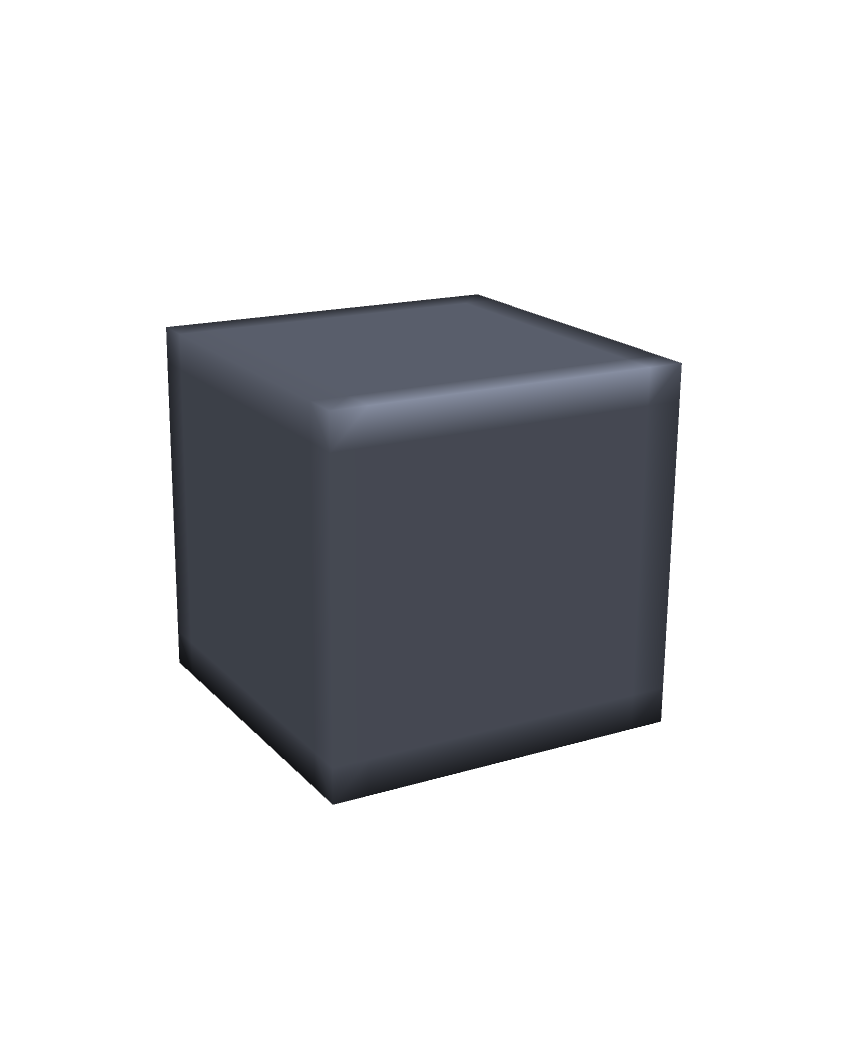
\includegraphics[width=0.24\textwidth]{resources/hexcli_00.png}
        \hfill
        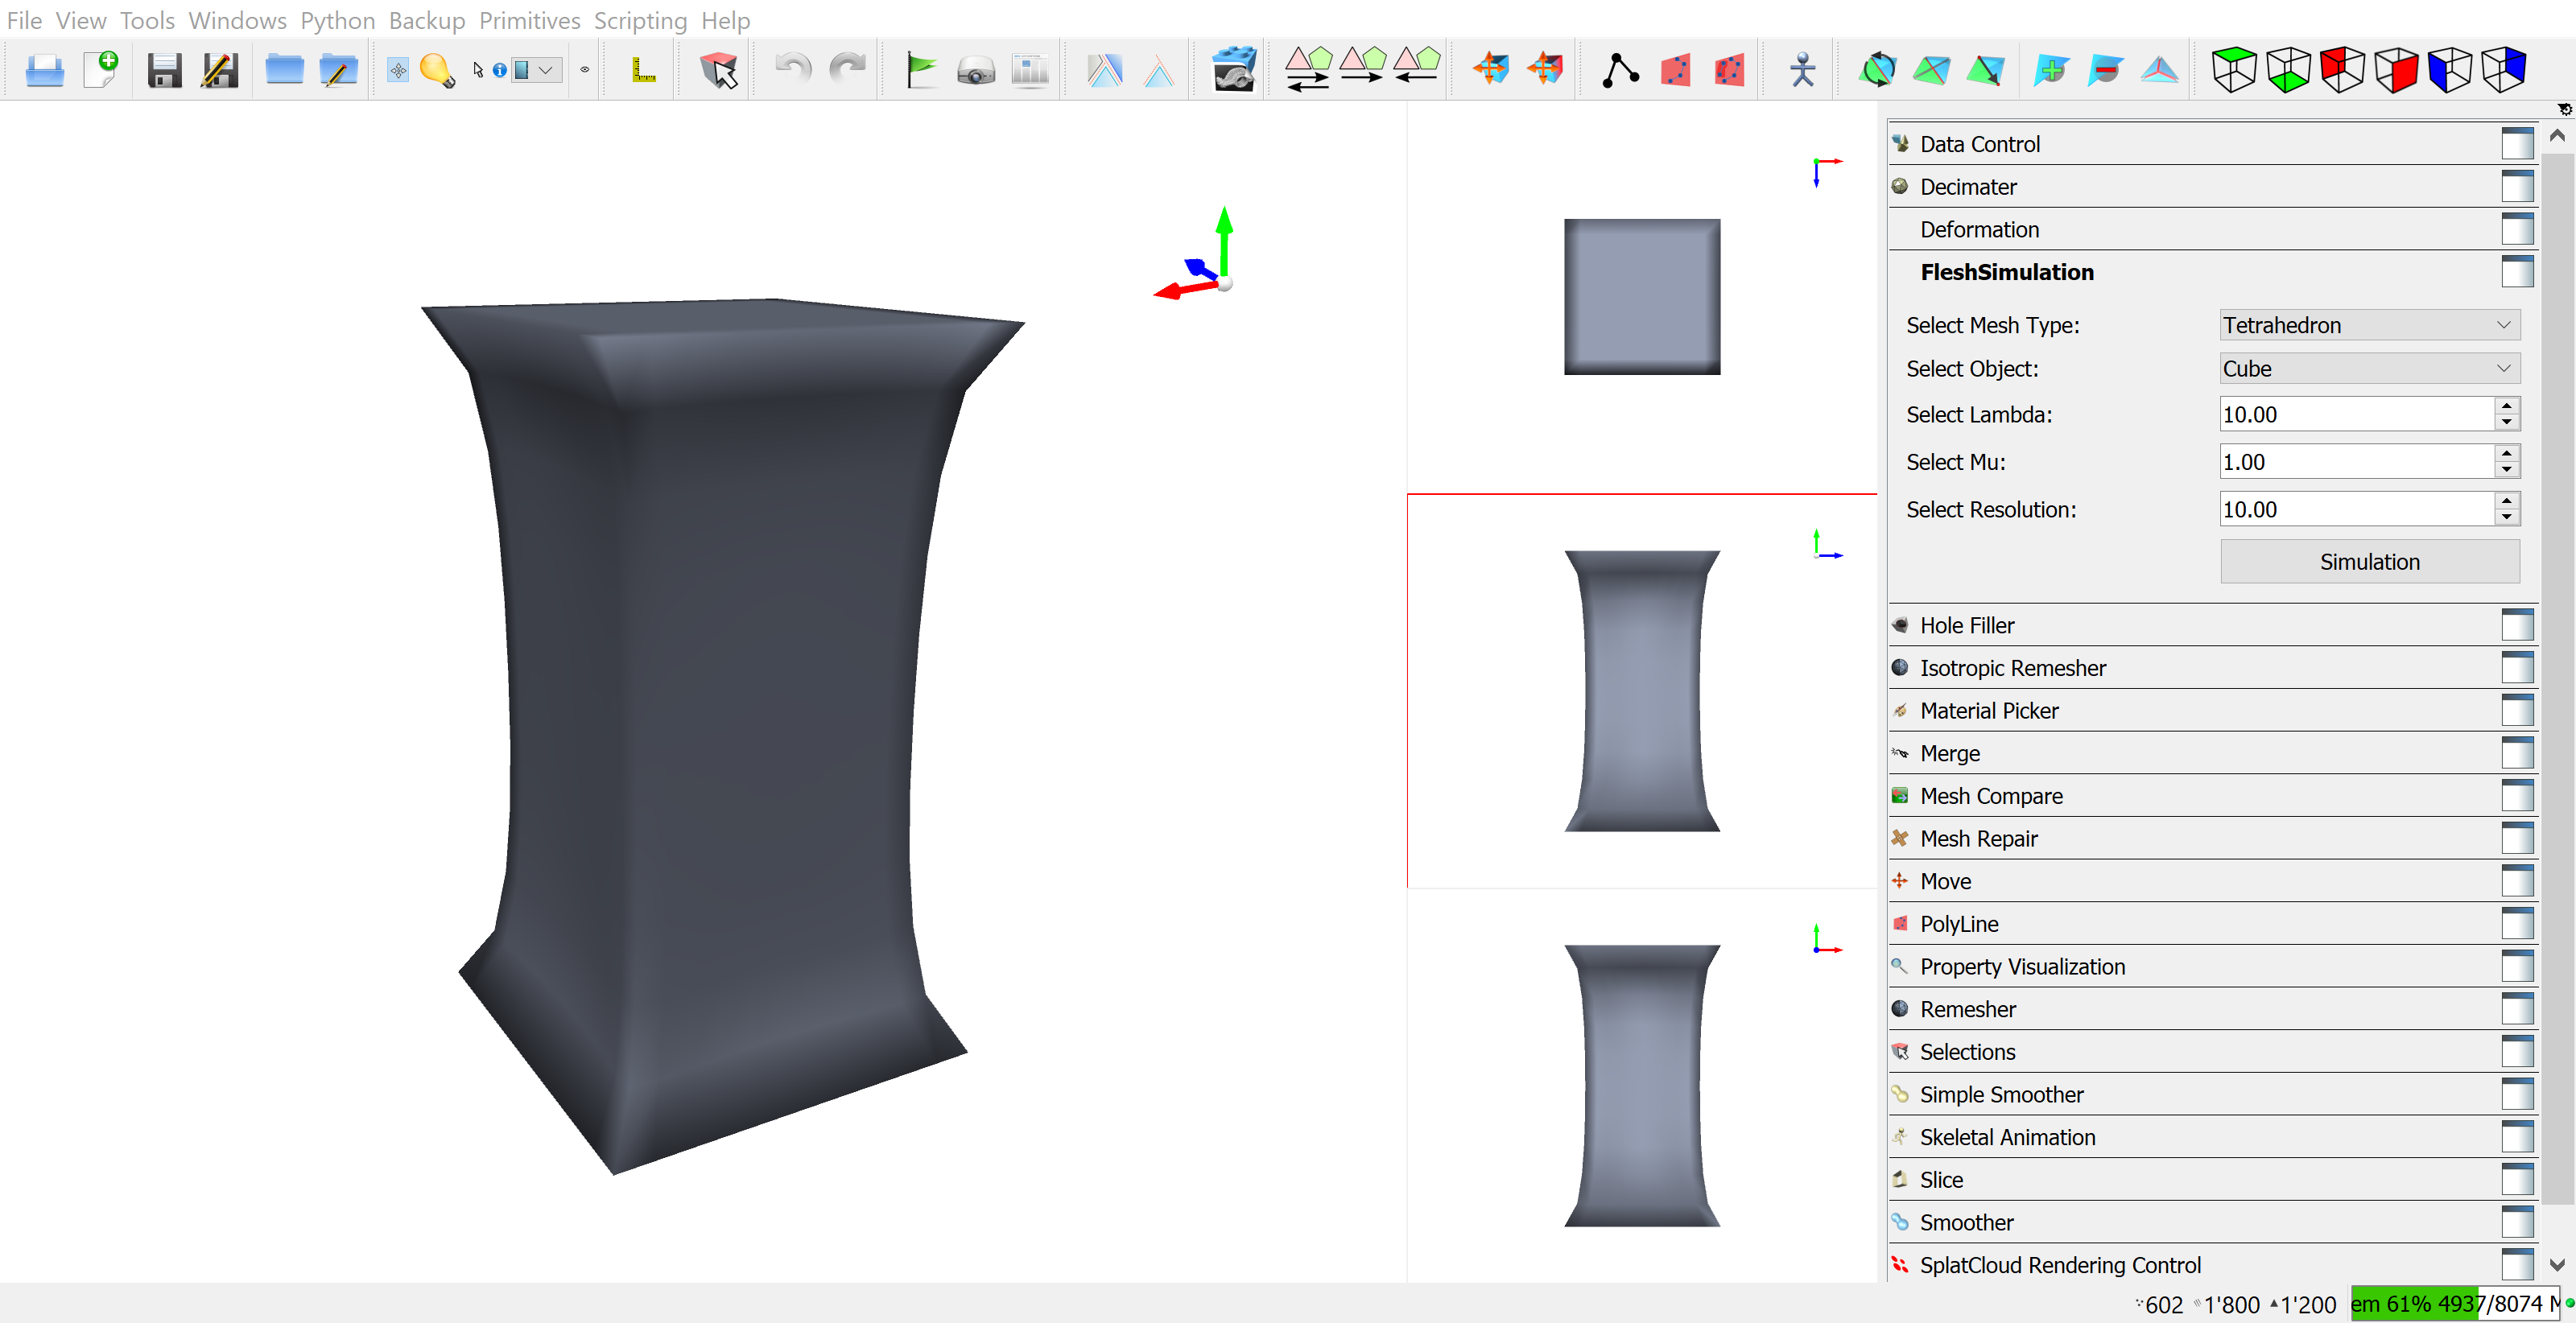
\includegraphics[width=0.24\textwidth]{resources/hexcli_08.png}
        \hfill
        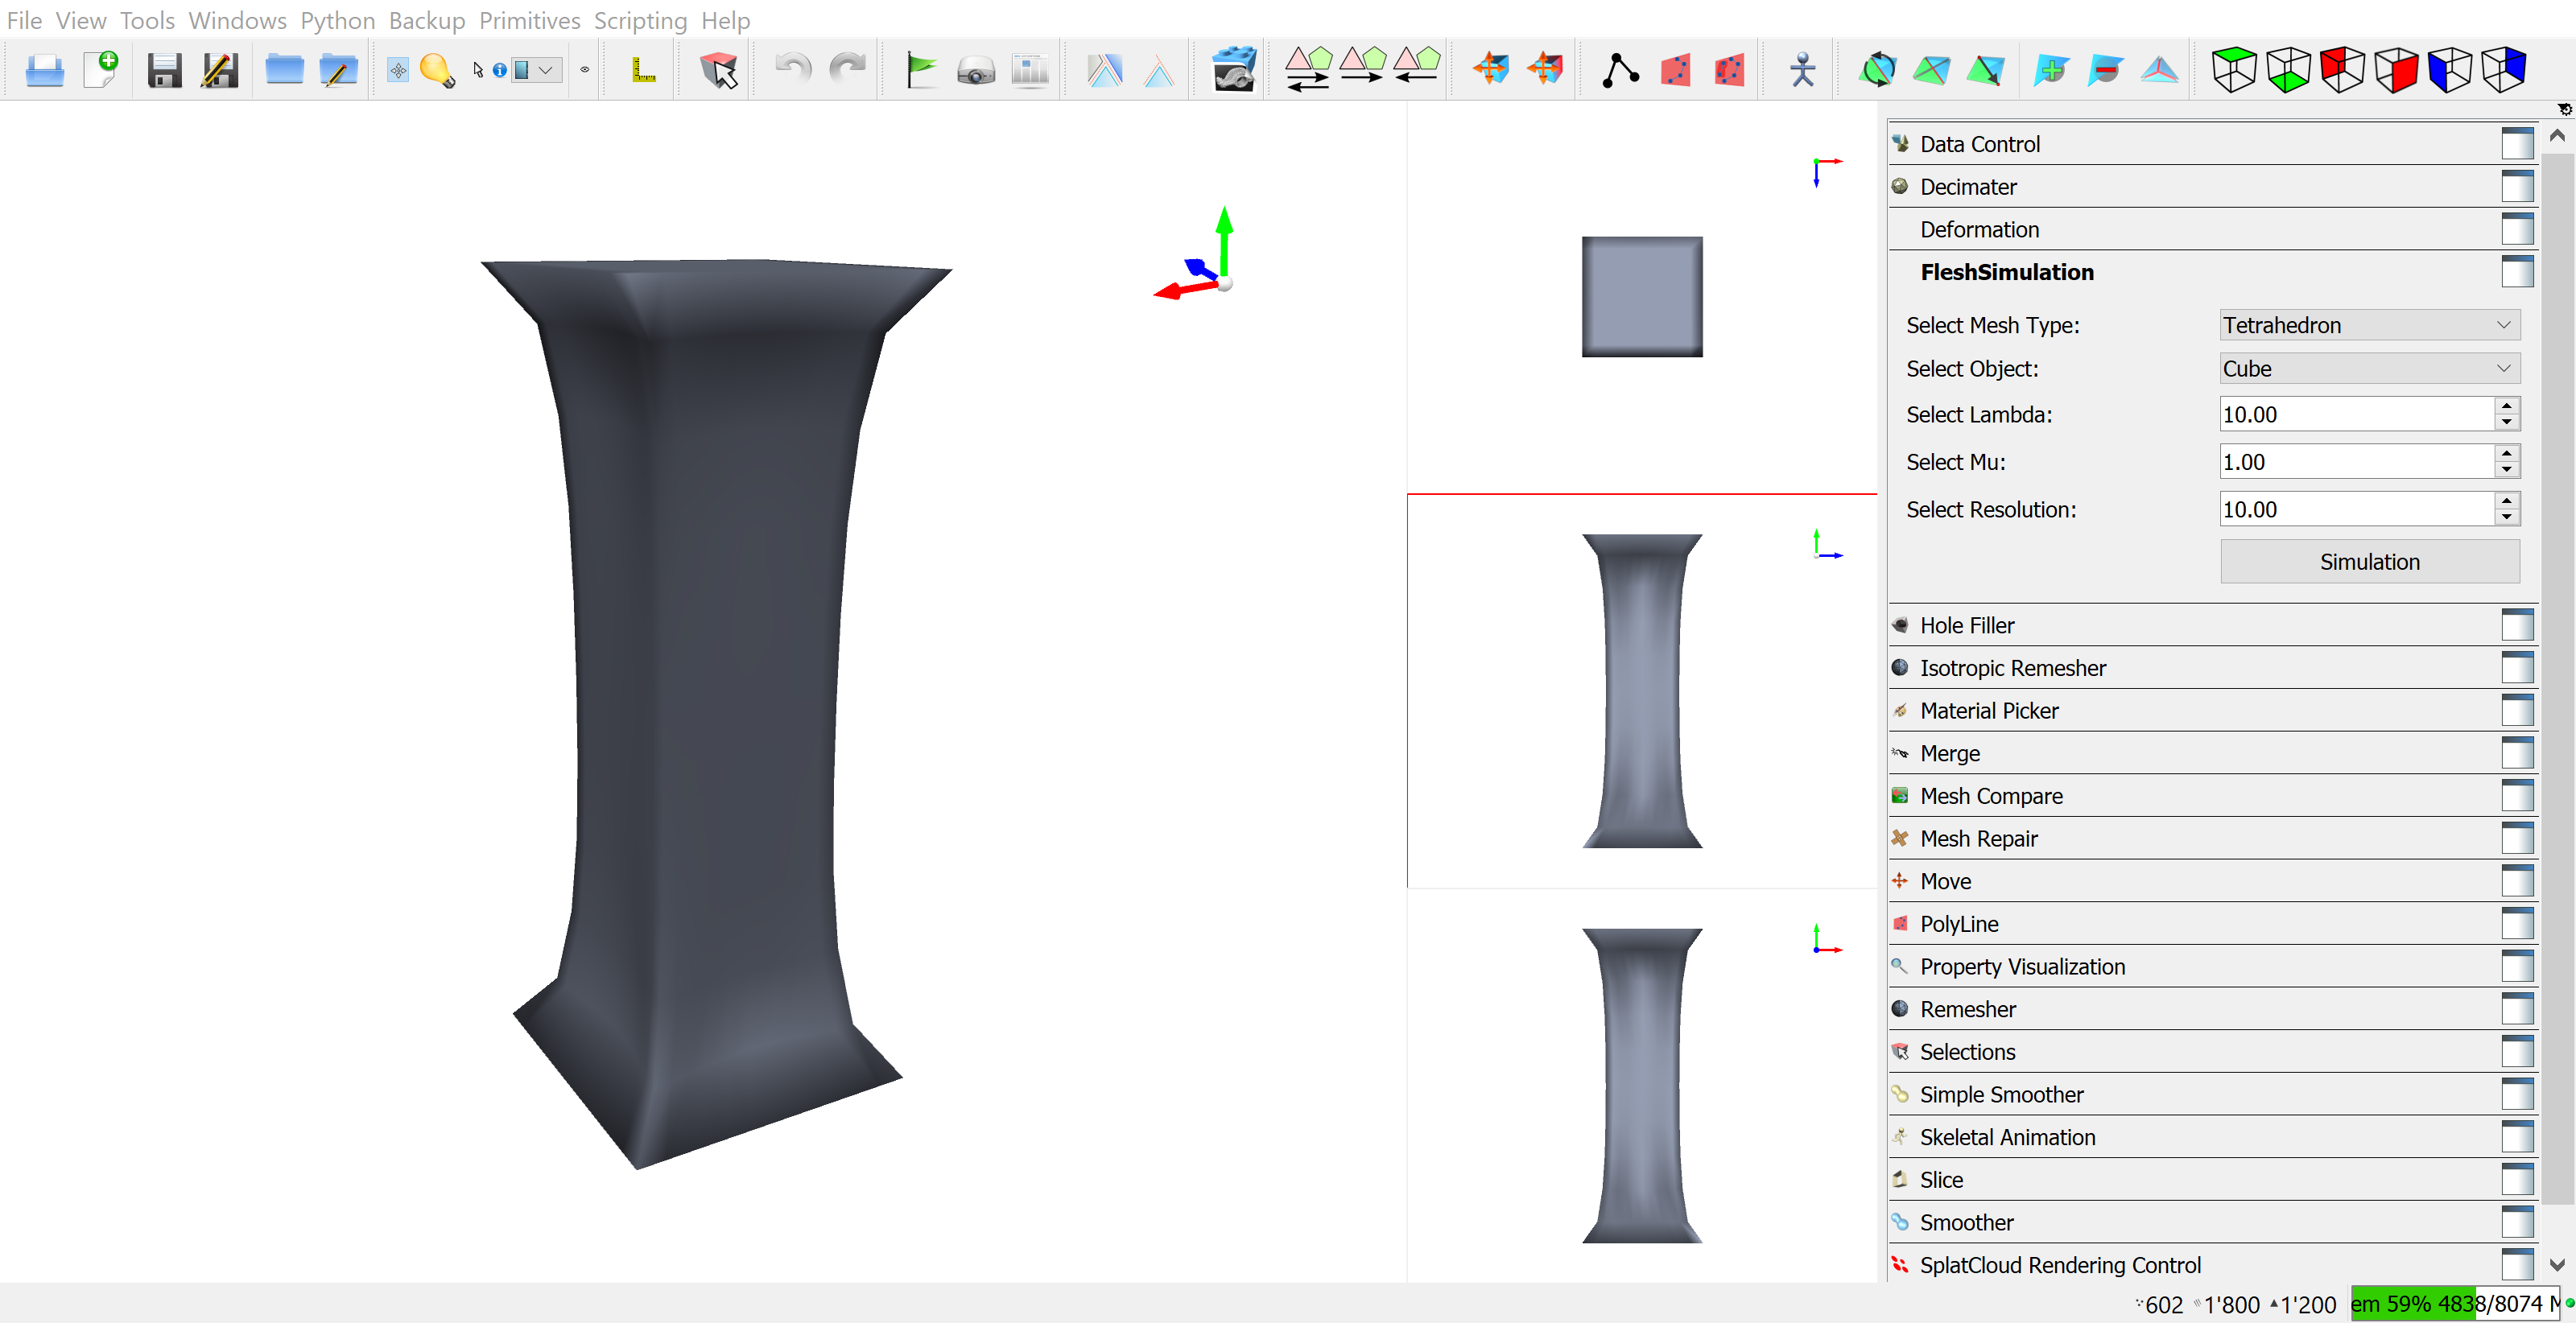
\includegraphics[width=0.24\textwidth]{resources/hexcli_16.png}
        \hfill
        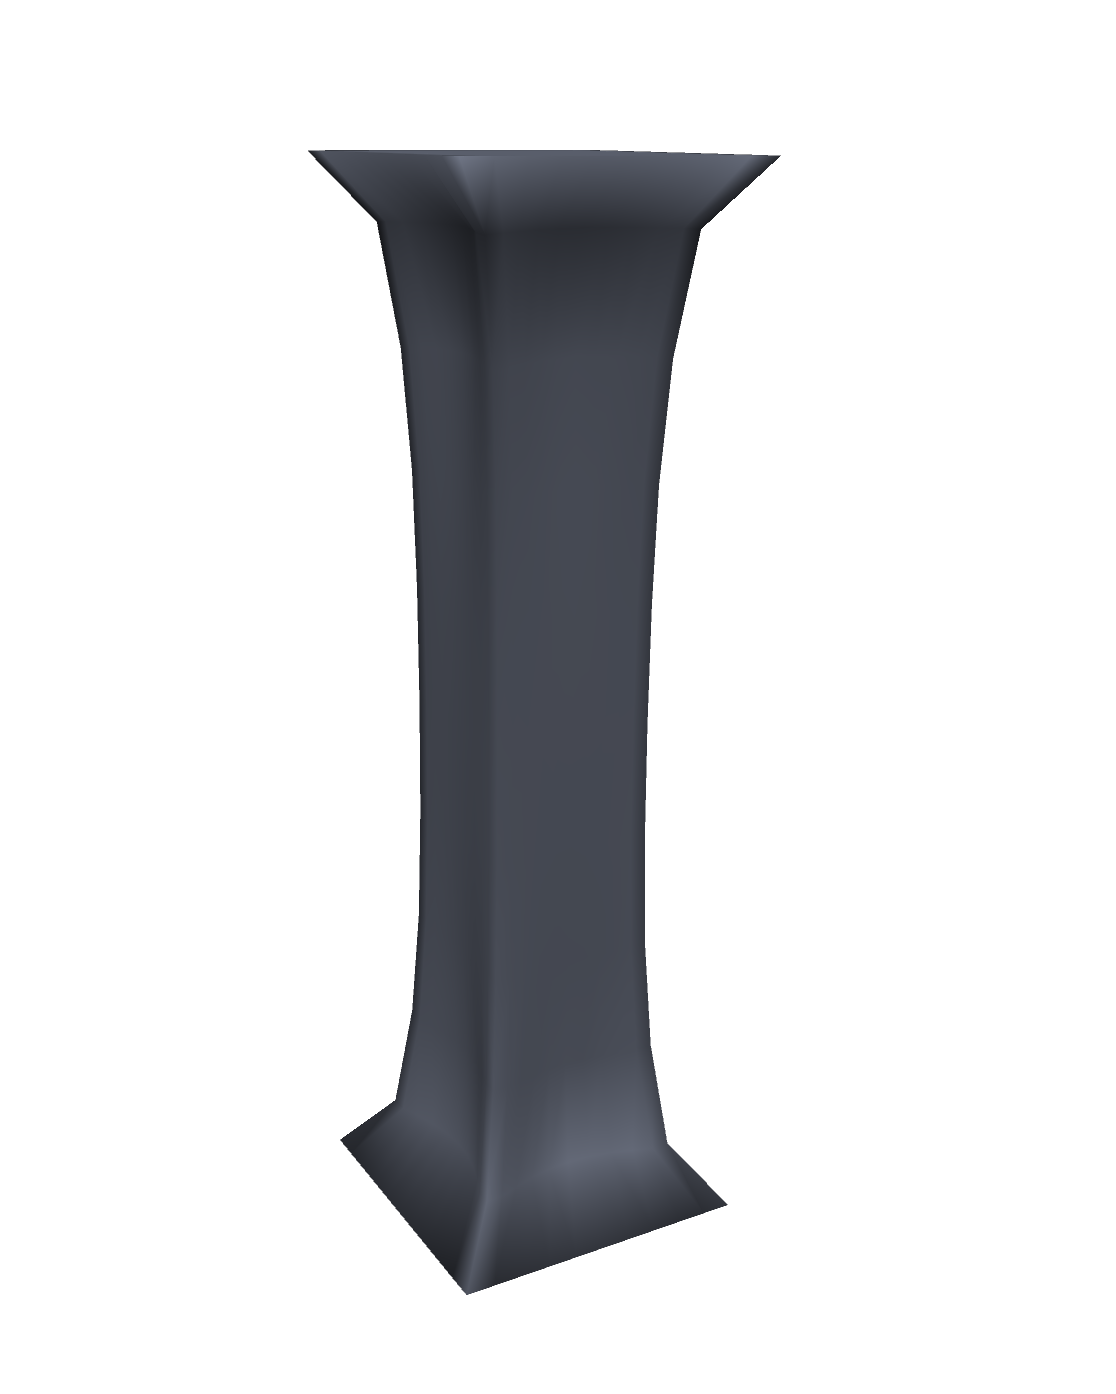
\includegraphics[width=0.24\textwidth]{resources/hexcli_24.png}
        \caption{Stretch test on a hexahedral mesh}
    \end{subfigure}
    \vskip\baselineskip
    \begin{subfigure}[b]{\textwidth}
        \centering
        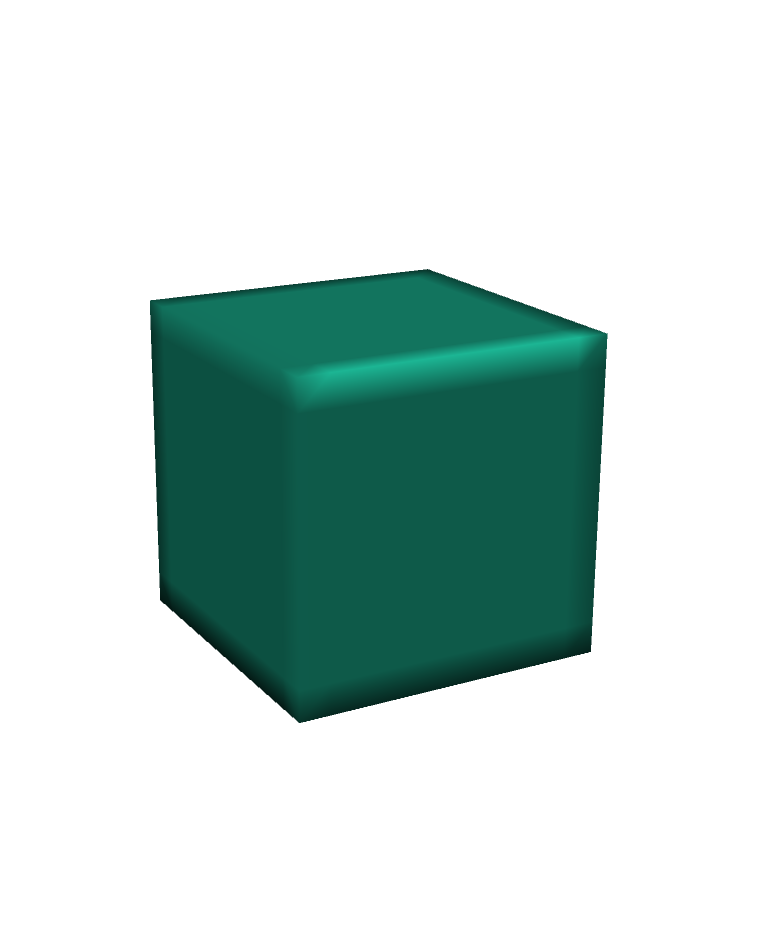
\includegraphics[width=0.24\textwidth]{resources/tetcli_00.png}
        \hfill
        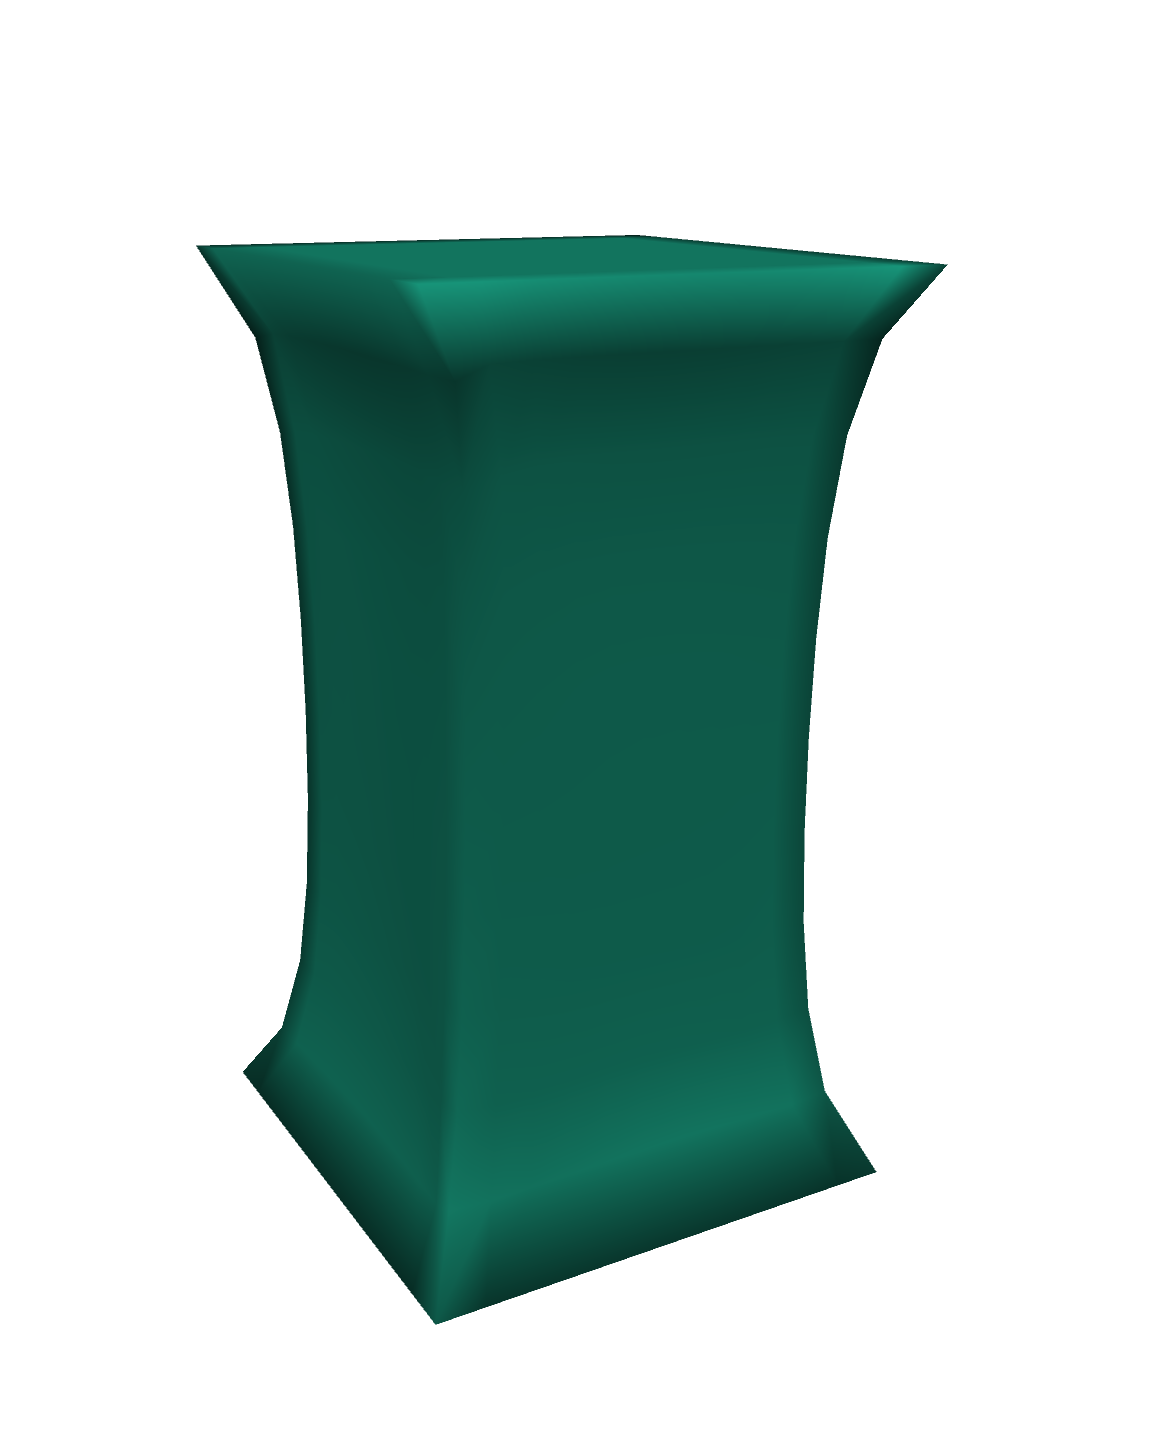
\includegraphics[width=0.24\textwidth]{resources/tetcli_08.png}
        \hfill
        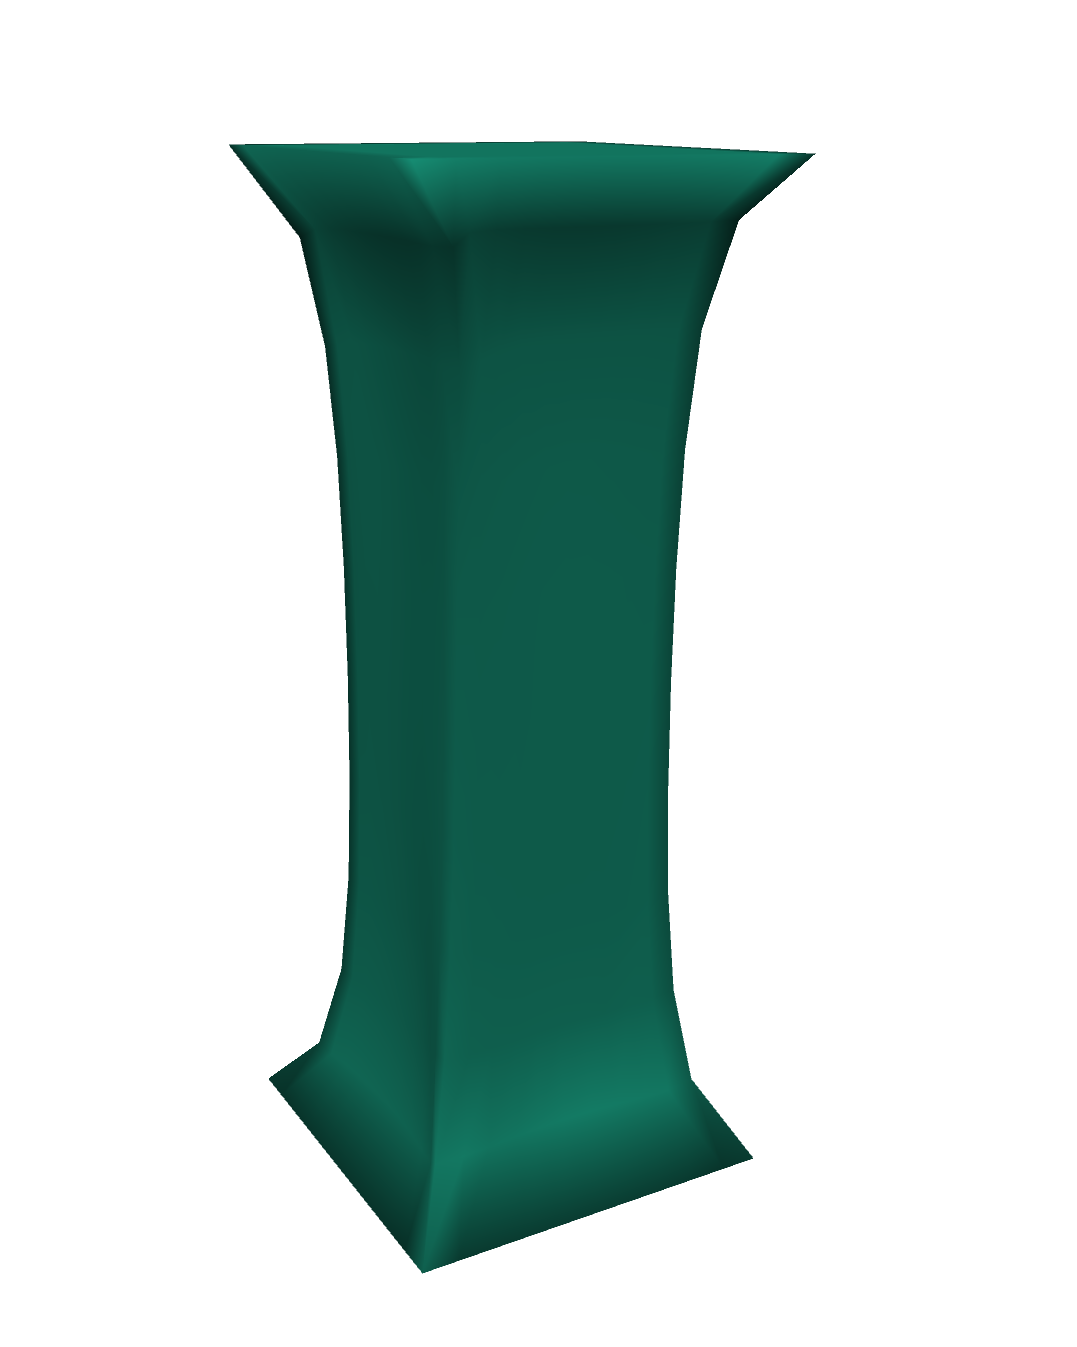
\includegraphics[width=0.24\textwidth]{resources/tetcli_16.png}
        \hfill
        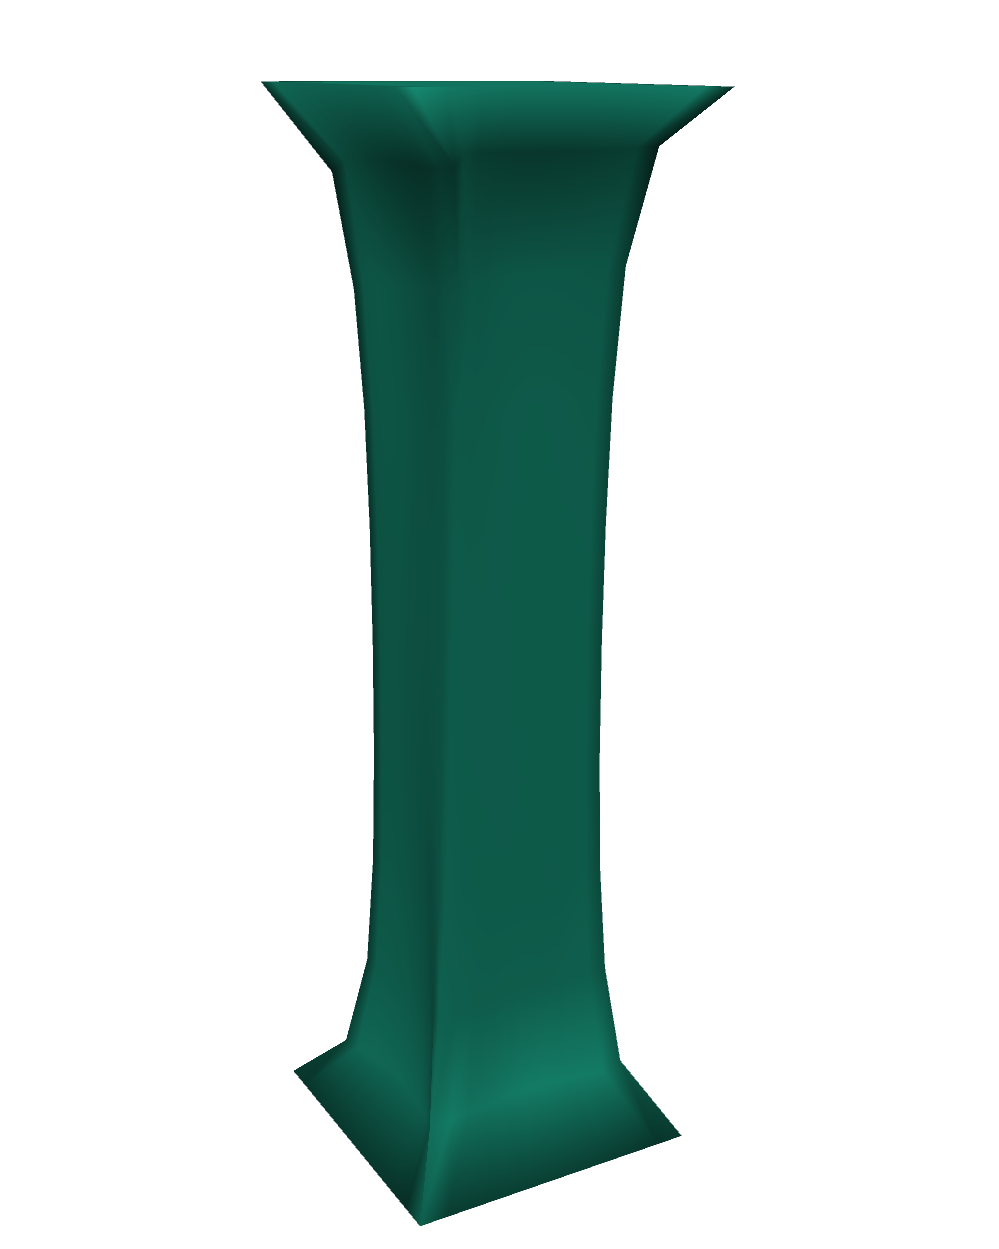
\includegraphics[width=0.24\textwidth]{resources/tetcli_24.png}
        \caption{Stretch test on a tetrahedral mesh}
    \end{subfigure}
    \caption[Stretch test performed on a cube]{Stretch test performed on a cube with (a) a hexahedral mesh and (b) a tetrahedral mesh}
    \label{fig:stretchtest}
\end{figure}

\subsection{Comparison of different input variables}
For examining the influence of the input variable, I experimented with different values. The importance of the resolution is straight forward. For a higher resolution, the cube consists of more vertices and edges. This results in smoother results but also a longer runtime. If we choose a resolution of $30$, the cube consists of $29'791$ vertices and $162'000$ tetrahedra respectively $27'000$ hexahedra. Table \ref{table:res_tet} and \ref{table:res_hex} show the completed Newton iterations. The amount of iterations is slightly more than in the example in section 3.4.1.

\begin{table}[!htbp]
\parbox{.45\linewidth}{
\centering
\begin{tabular}{ | l | l |}
\hline
\textbf{Step size} & \textbf{Iterations} \\ \hline
1-7 & 2 \\ \hline
8-13 & 3 \\ \hline
14-20 & 4 \\ \hline
21-25 & 5 \\ \hline
\end{tabular}
\caption{Newton iterations for a tetrahedral mesh (res=30)}
\label{table:res_tet}
}
\hfill
\parbox{.45\linewidth}{
\centering
\begin{tabular}{ | l | l |}
\hline
\textbf{Step size} & \textbf{Iterations} \\ \hline
1-4 & 3 \\ \hline
5-10 & 4 \\ \hline
11-15 & 5 \\ \hline
16-19 & 6 \\ \hline
20-23 & 7 \\ \hline
24-25 & 8 \\ \hline
\end{tabular}
\caption{Newton iterations for a hexahedral mesh (res=30)}
\label{table:res_hex}
}
\end{table}

Fig. \ref{fig:res} shows the results with a higher resolution of $30$ compared to a lower resolution of $10$. All other input variables are the same. The figure shows the results of the deformation step $25$. We can see that a higher resolution clearly gives us much nicer results.

\begin{figure}[!ht]
\centering
\begin{subfigure}{.47\textwidth}
  \centering
  % include first image
  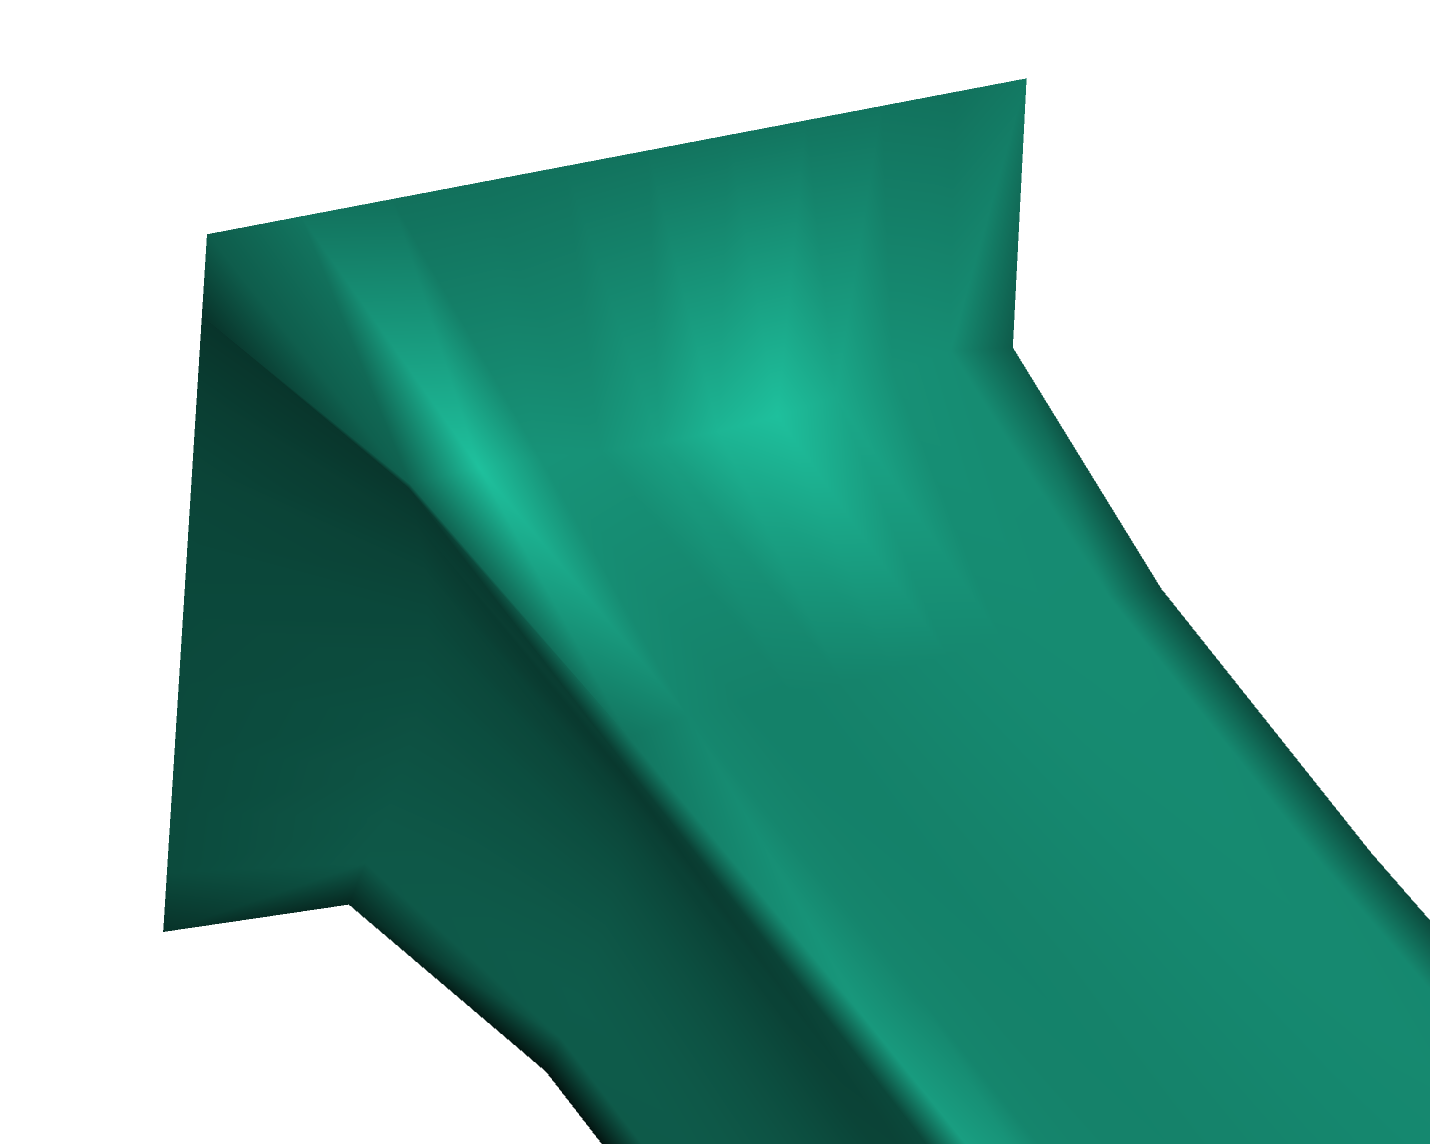
\includegraphics[width=.8\linewidth]{resources/default_zoom_tet.png}  
  \caption{Step 25 with a resolution of 10}
  \label{fig:res_1}
\end{subfigure}
\begin{subfigure}{.47\textwidth}
  \centering
  % include second image
  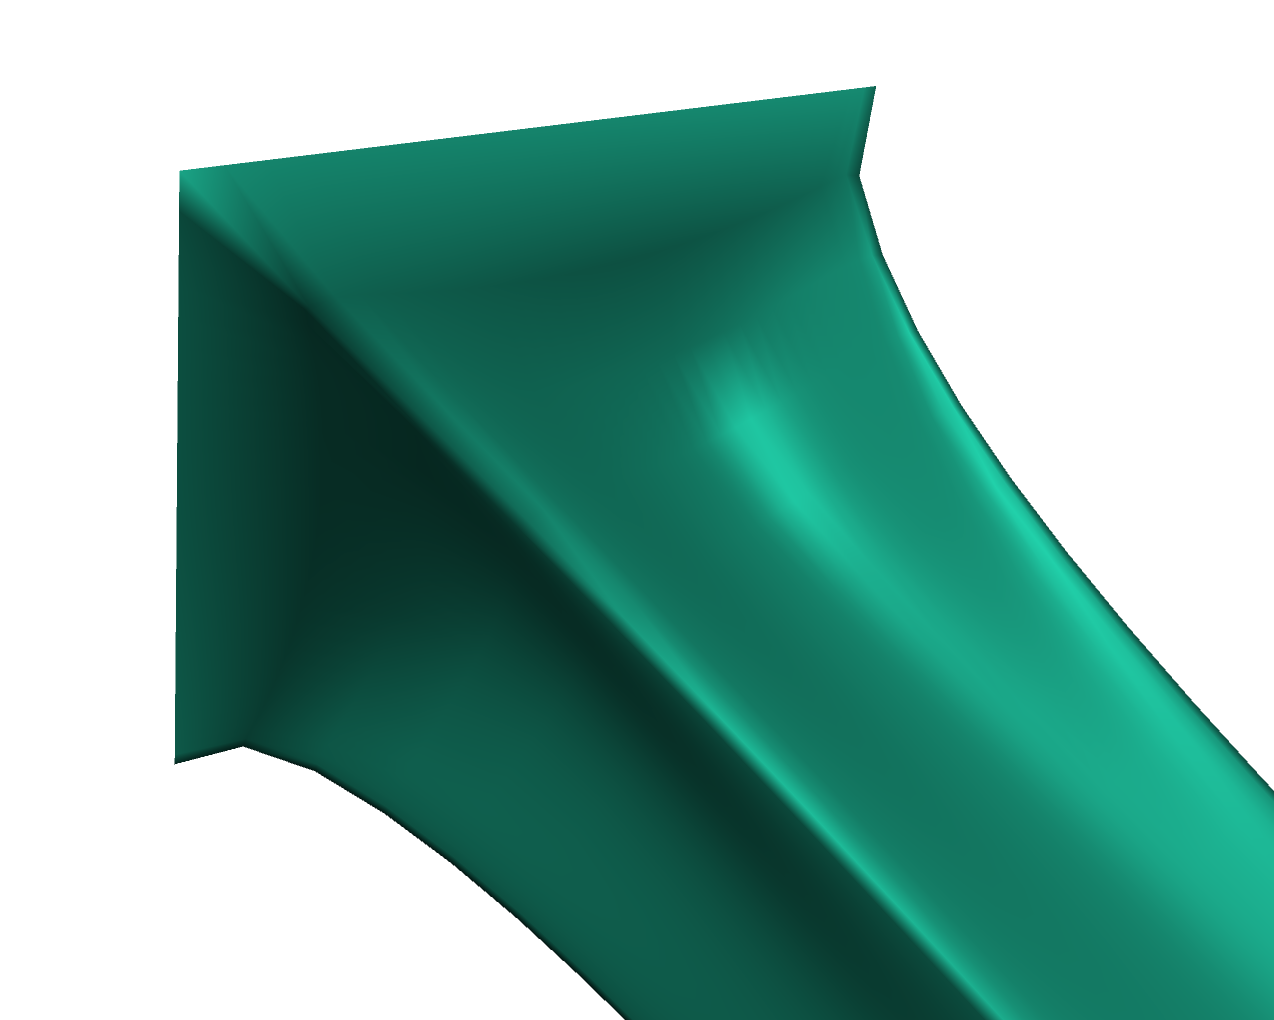
\includegraphics[width=.8\linewidth]{resources/res_zoom_tet.png}  
  \caption{Step 25 with a resolution of 30}
  \label{fig:res_2}
\end{subfigure}
\caption{Results with a different resolution on a tetrahedral mesh}
\label{fig:res}
\end{figure}


In addition, we can increase or decrease \textit{\mu} and \textit{\lambda} which changes the poisson's ratio. If we decrease \textit{\lambda}, the poisson's ratio also decreases. We can set \textit{\lambda} equal to $1.0$ and let the other variables stay the same as in the last example (\textit{\mu} $= 1.0$, resolution $= 30.0$). Fig. \ref{fig:lambda} shows how the deformation is influenced by changing $\lambda$. With these inputs the cube gets wider in the middle part, as the poisson's ratio indicates that the material is more resistant to the stretching.

\begin{figure}[!ht]
\centering
\begin{subfigure}{.47\textwidth}
  \centering
  % include first image
  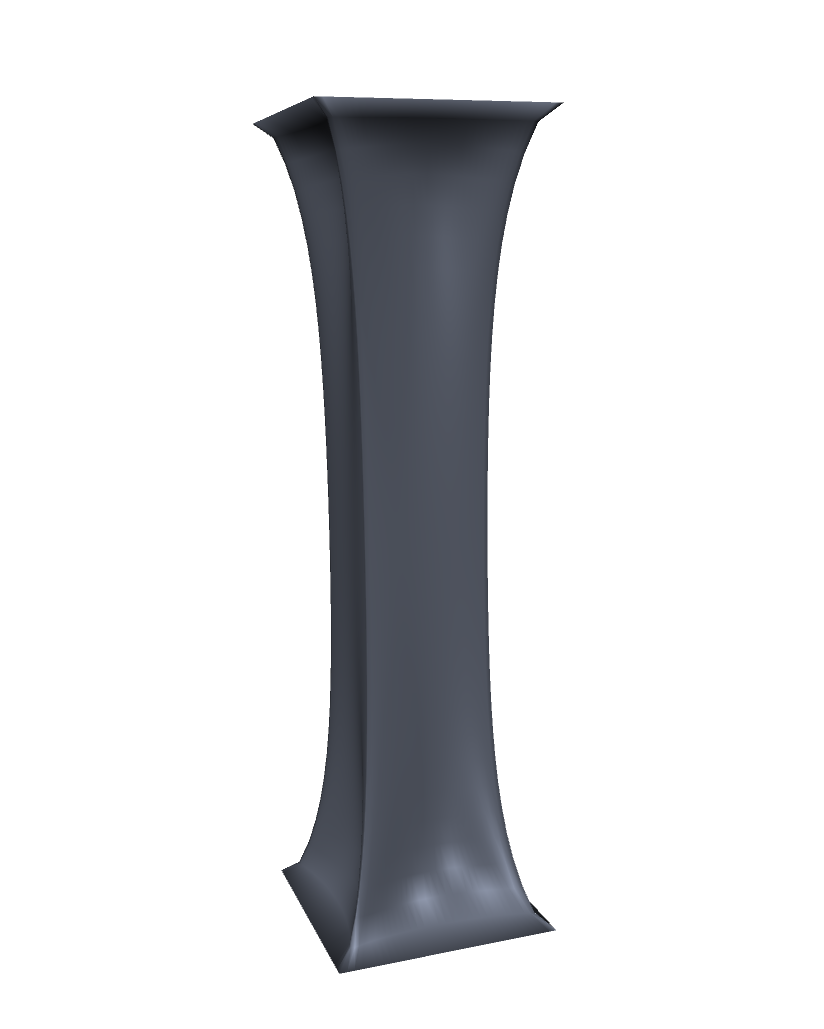
\includegraphics[width=.8\linewidth]{resources/lambda_comparison_res.png}  
  \caption{Step 25 with $\lambda = 10.0$}
  \label{fig:lambda_1}
\end{subfigure}
\begin{subfigure}{.47\textwidth}
  \centering
  % include second image
  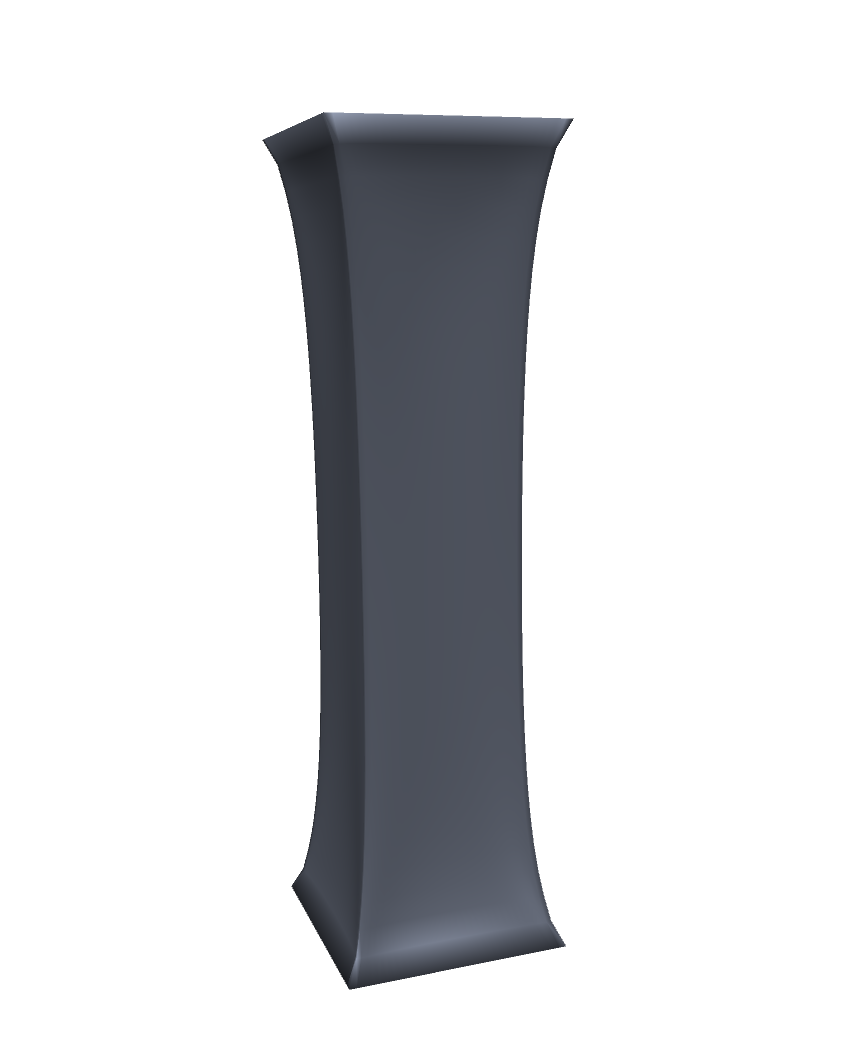
\includegraphics[width=.8\linewidth]{resources/lambda_comparison_lambda.png}  
  \caption{Step 25 with $\lambda = 1.0$}
  \label{fig:lambda_2}
\end{subfigure}
\caption{Results with a different values for $\lambda$ on a hexahedral mesh}
\label{fig:lambda}
\end{figure}

Table \ref{table:lambda_tet} and \ref{table:lambda_hex} show the amount of Newton iteration needed for the chosen input values. The amount of iterations has decreased for both meshes. We need less iterations because the extend of the deformation is smaller.

\begin{table}[!htbp]
\parbox{.45\linewidth}{
\centering
\begin{tabular}{ | l | l |}
\hline
\textbf{Step size} & \textbf{Iterations} \\ \hline
1-25 & 2 \\ \hline
\end{tabular}
\caption{Newton iterations for a tetrahedral mesh ($\lambda = 1.0$)}
\label{table:lambda_tet}
}
\hfill
\parbox{.45\linewidth}{
\centering
\begin{tabular}{ | l | l |}
\hline
\textbf{Step size} & \textbf{Iterations} \\ \hline
1-25 & 3 \\ \hline
\end{tabular}
\caption{Newton iterations for a hexahedral mesh ($\lambda = 1.0$)}
\label{table:lambda_hex}
}
\end{table}

Now instead of decreasing the poisson's ratio, let's increase it. We can achieve that by choosing $\mu = 0.1$ and letting the other variables stay the same as in the first example of this section ($\lambda = 10.0$, res $= 10$). This is an extreme case because the poisson's ratio is very close to $0.5$. A higher poisson's value makes the cube more susceptible for stretching. We can see this effect a bit by comparing the two images in Fig. \ref{fig:mu}, although the difference is not extreme. The model still behaves well and no artefacts can be seen.

\begin{figure}[!ht]
\centering
\begin{subfigure}{.47\textwidth}
  \centering
  % include first image
  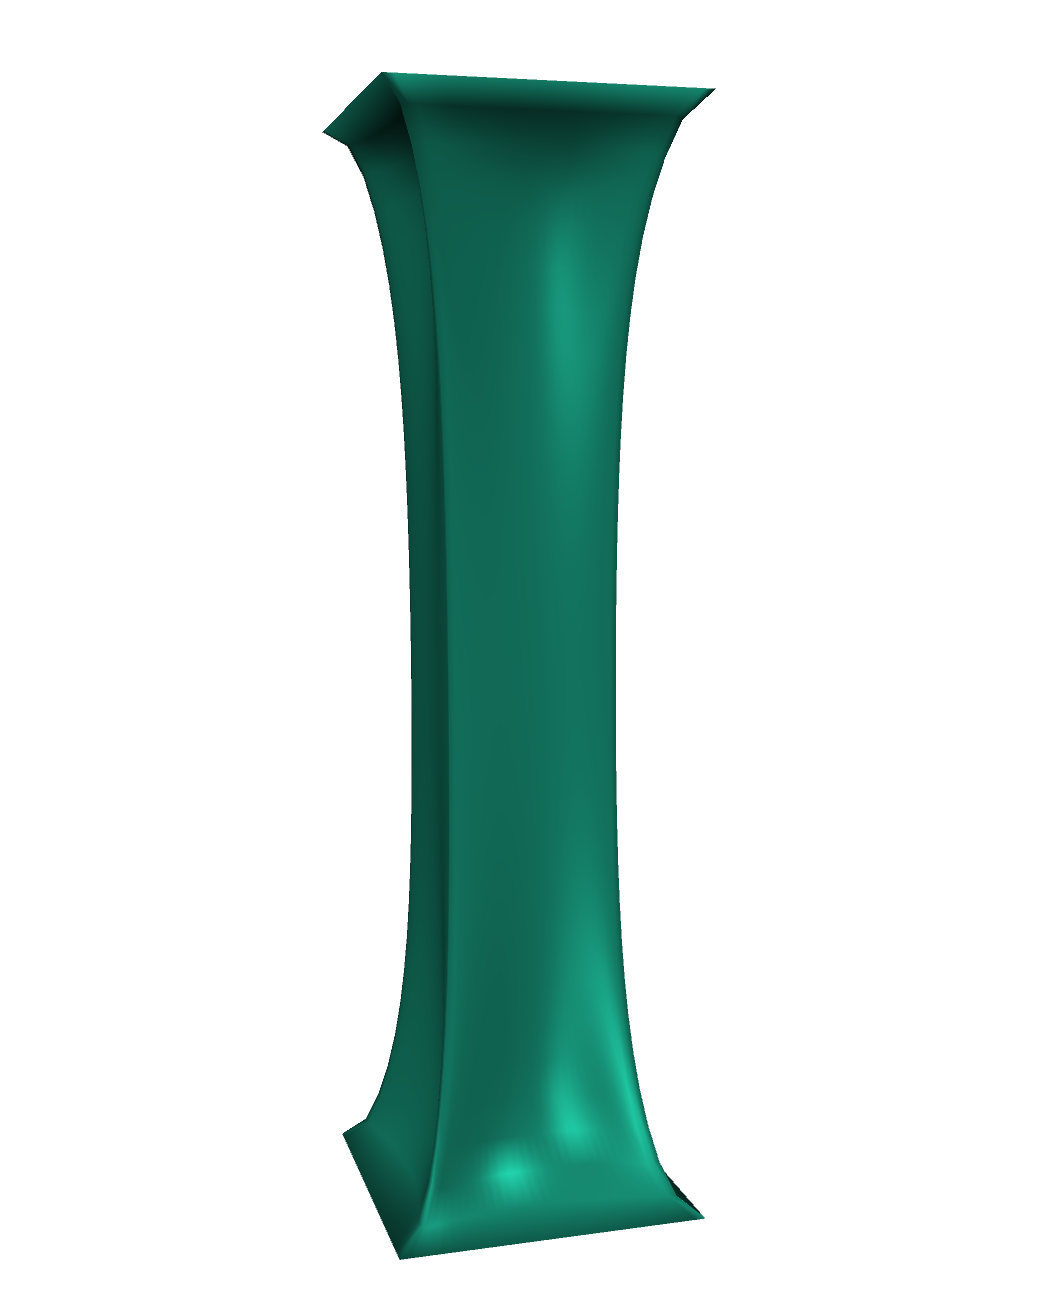
\includegraphics[width=.8\linewidth]{resources/mu_res_new.png}  
  \caption{Step 25 with $\mu = 1.0$}
  \label{fig:mu_1}
\end{subfigure}
\begin{subfigure}{.47\textwidth}
  \centering
  % include second image
  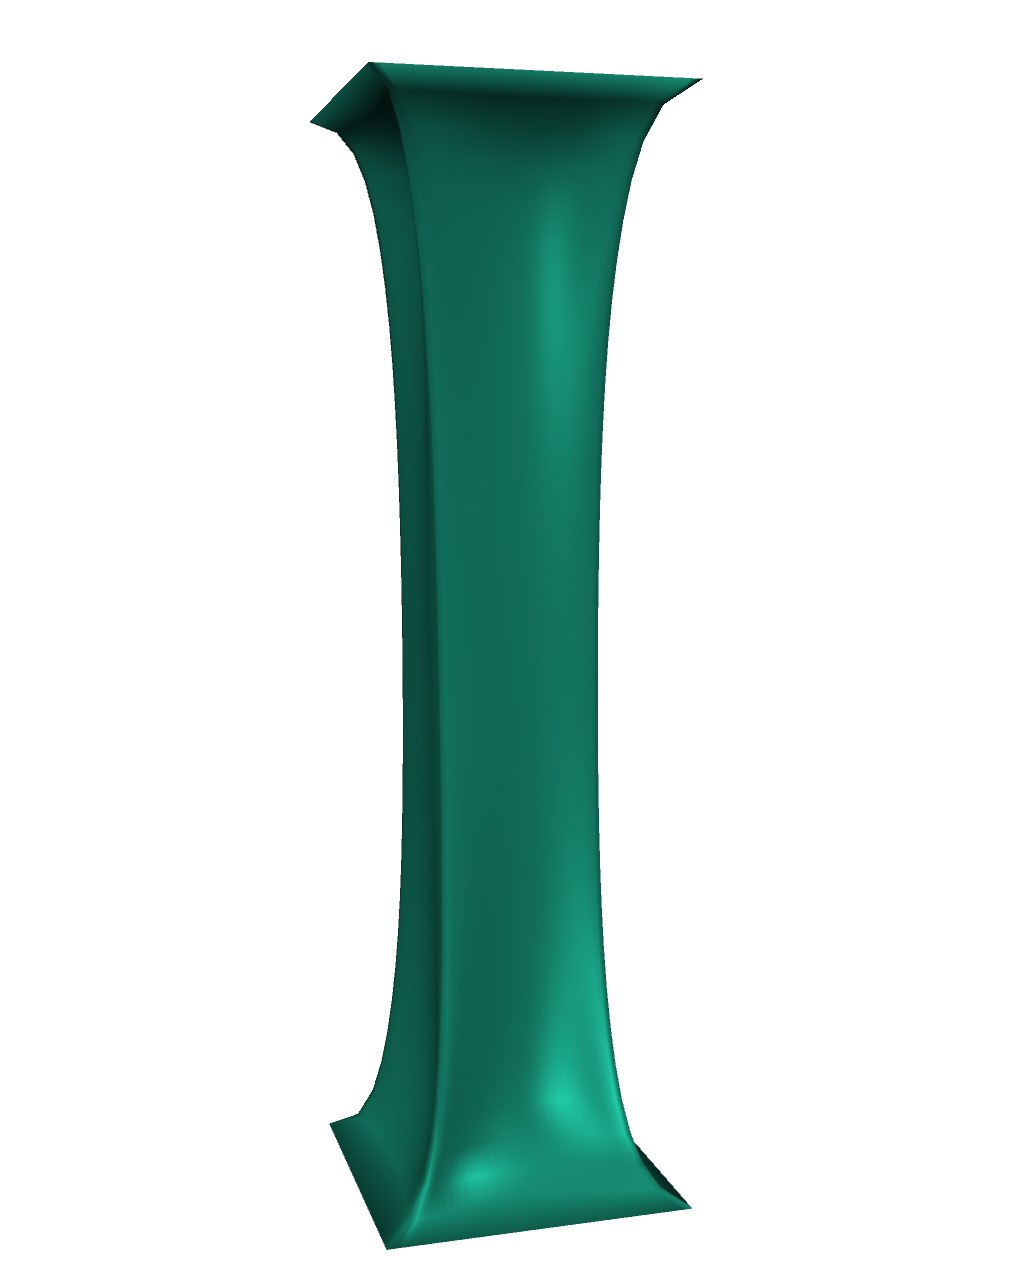
\includegraphics[width=.8\linewidth]{resources/mu_mu_new.png}  
  \caption{Step 25 with $\mu = 0.1$}
  \label{fig:mu_2}
\end{subfigure}
\caption{Results with a different values for $\mu$ on a tetrahedral mesh}
\label{fig:mu}
\end{figure}

For solving this system, we need more Newton iterations as we can see in Table \ref{table:mu_tet}  and \ref{table:mu_hex}. This is caused by the more complex deformation. The cube gets narrower in the middle part which increases the difficulty of reaching a valid solution.
\begin{table}[!htbp]
\parbox{.45\linewidth}{
\centering
\begin{tabular}{ | l | l |}
\hline
\textbf{Step size} & \textbf{Iterations} \\ \hline
1 & 2 \\ \hline
2-3 & 3 \\ \hline
4-6 & 4 \\ \hline
7 & 5 \\ \hline
8-11 & 6 \\ \hline
12 & 7 \\ \hline
13-20 & 8 \\ \hline
21-25 & 10 \\ \hline
\end{tabular}
\caption{Newton iterations for a tetrahedral mesh ($\mu = 0.1$)}
\label{table:mu_tet}
}
\hfill
\parbox{.45\linewidth}{
\centering
\begin{tabular}{ | l | l |}
\hline
\textbf{Step size} & \textbf{Iterations} \\ \hline
1 & 5 \\ \hline
2 & 6 \\ \hline
3 & 7 \\ \hline
4 & 8 \\ \hline
5-6 & 9 \\ \hline
7 & 10 \\ \hline
8-9 & 11 \\ \hline
10-11 & 12 \\ \hline
12 & 13 \\ \hline
13-14 & 14 \\ \hline
15 & 15 \\ \hline
16 & 16 \\ \hline
17-19 & 17 \\ \hline
20-25 & 19 \\ \hline
\end{tabular}
\caption{Newton iterations for a hexahedral mesh ($\mu = 0.1$)}
\label{table:mu_hex}
}
\end{table}


\subsubsection{Extreme values}
We can test the energy with some extreme values. For getting a very low poisson's value near 0, I choose $\lambda = 0.1$ and $\mu = 10.0$ with a resolution of $30$. This takes about $100$ to $200$ Newton iterations. The finished result gives us a strange looking deformations and little artefacts as shown in Fig. \ref{fig:mu_extreme}. This does not mean that it is a bad model, but rather that is only suited for higher poisson's ratio like it is the case for simulating flesh.

\begin{figure}[!htbp]
	\centering
	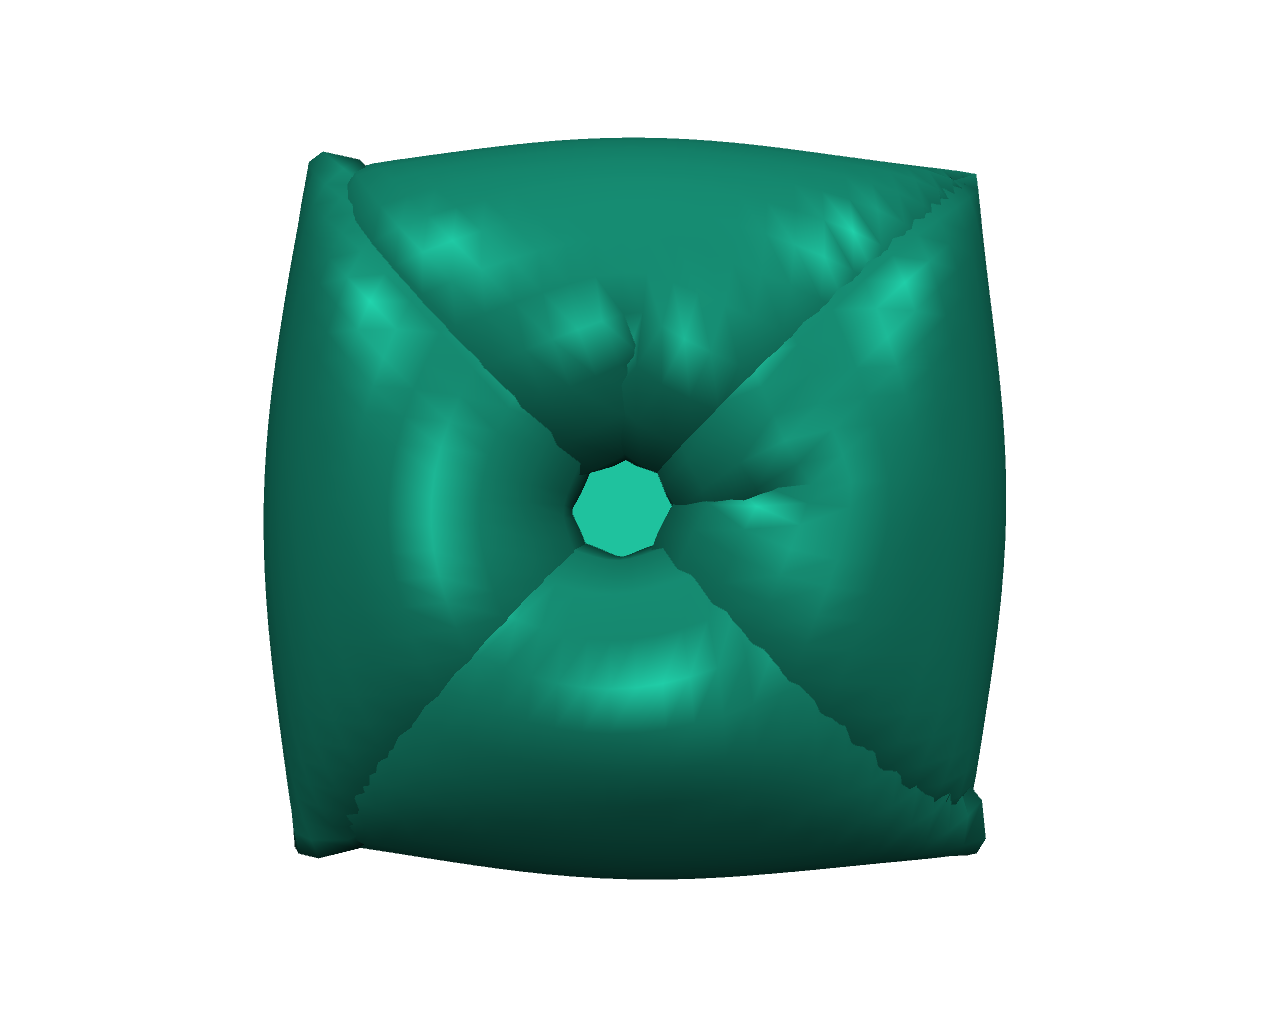
\includegraphics[width=0.5\textwidth]{resources/mu_extreme_1.png}
	\caption{Step 4 with $\lambda = 0.1$ and $\mu = 10.0$ on a tetrahedral mesh shown from above}
	\label{fig:mu_extreme}
\end{figure}


\newpage

\section{Discussion}
Stuff, Taylor approx.

\todoredefined[inline]{
TODO: Explain difference in iteration with meshes. Explain artefacts.
}


